%! TEX root = applsci-4501207.tex
%  LaTeX support: latex@mdpi.com
%  For support, please attach all files needed for compiling as well as the log file, and specify your operating system, LaTeX version, and LaTeX editor.

%=================================================================
\documentclass[applsci,article,submit,moreauthors]{Definitions/mdpi}
\usepackage{placeins}
%\pagestyle{empty}  % 全局无页眉页脚
%\documentclass[preprints,article,submit,moreauthors]{Definitions/mdpi} 
% For posting an early version of this manuscript as a preprint, you may use "preprints" as the journal. Changing "submit" to "accept" before posting will remove line numbers.

%--------------------
% Class Options:
%--------------------
%----------
% journal
%----------
% Choose between the following MDPI journals:
% accountaudit, acn, acoustics, actuators, addictions, addictprev, adhesives, adolescents, aerobiology, aerospace, agriculture, agriengineering, agrochemicals, agronomy, ai, aichem, aieng, aimater, aimed, aipa, air, aisens, aisoc, algorithms, allergies, alloys, amh, analog, analytica, analytics, anatomia, anesthres, animals, antibiotics, antibodies, antioxidants, applbiosci, appliedchem, appliedmath, appliedphys, applmech, applmicrobiol, applnano, applsci, aps, aquacj, archaeolstud, architecture, arm, arthropoda, asc, asi, astronautics, astronomy, atmosphere, atoms, audiolres, automation, axioms, bacteria, batteries, bdcc, beverages, biochem, bioengineering, biologics, biology, biomass, biomechanics, biomed, biomedicines, biomedinformatics, biomimetics, biomolecules, biophysica, bioresourbioprod, biosensors, biosphere, biotech, birds, blockchains, bloods, blsf, brainsci, breath, buildings, cancers, carbon, cardio, cardiogenetics, cardiovascmed, catalysts, cells, ceramics, challenges, chemengineering, chemistry, chemosensors, chemproc, children, chips, cimb, civileng, cleantechnol, climate, clinbioenerg, clinpract, clockssleep, cmd, cmtr, coasts, coatings, colloids, colorants, commodities, complexities, complications, compounds, computation, computers, condensedmatter, conservation, constrmater, cosmetics, covid, crops, cryo, cryptography, crystals, csmf, ctn, culture, curroncol, cyber, dairy, data, ddc, dentistry, dermato, dermatopathology, designs, devices, dhi, diabetology, diagnostics, dietetics, digital, disabilities, diseases, diversity, dna, drones, drugreact, drylands, dynamics, earth, ebj, ecm, ecologies, edm, eesp, electricity, electrochem, electronicmat, electronics, embodiedintell, encyclopedia, endocrines, energies, eng, engproc, entomology, entropy, environments, environremediat, epidemiologia, epigenomes, esa, est, fermentation, fibers, fintech, fire, fishes, fluids, foodeng, foods, forecasting, forensicsci, forests, fossstud, foundations, fractalfract, freshwater, fuels, future, futureinternet, futurepharmacol, futurephys, futuretransp, galaxies, gases, gastroent, gastrointestdisord, gastronomy, gels, genes, geochem, geographies, geohazards, geomatics, geometry, geosciences, geotechnics, geriatrics, germs, glacies, grainsci, grasses, green, greenhealth, gucdd, gynecolcancer, hardware, hazardousmatters, healthcare, healthcmater, hearts, hemato, hematolrep, hep, heritage, higheredu, highthroughput, horticulturae, hospitals, hydrobiology, hydrogen, hydrology, hydrometeorology, hydropower, hygiene, idr, iic, ijem, ijerph, ijgi, ijmd, ijms, ijns, ijom, ijp, ijpb, ijt, ijtm, ijtpp, ijtst, ime, immuno, industries, inflammj, informatics, information, infrastructures, inorganics, insects, instruments, inventions, iot, j, jaestheticmed, jal, japma, jcdd, jcm, jcp, jcrm, jcs, jcto, jdad, jdb, jdream, jemr, jeta, jfb, jfmk, jfth, jgbg, jgg, jimaging, jlpea, jmahp, jmmp, jmms, jmp, jmse, jne, jnt, jof, joi, joitmc, joma, jop, joptm, jor, jox, jpbi, jphytomed, jpm, jsan, jtaer, jvd, jzbg, kidneydial, kinasesphosphatases, knowledge, labmed, laboratories, lam, land, lasers, legumes, life, lights, limnolrev, lipidology, liquids, livers, logics, logistics, lubricants, lymphatics, machines, macromol, magnetism, magnetochemistry, make, marinedrugs, maritime, materials, materproc, mathematics, mca, mcb, measurements, medicina, medicines, medsci, membranes, merits, metabolites, metals, meteorology, methane, metrics, metrology, micro, microarrays, microbiolres, microelectronics, micromachines, microorganisms, microplastics, microwave, minerals, mining, mmphys, modelling, molbank, molecules, mollusca, mps, msf, mti, multimedia, muscles, nanoenergyadv, nanomanufacturing, nanomaterials, ncrna, ndt, network, neuroglia, neuroimaging, neurolint, neurosci, nitrogen, notspecified, nursrep, nutraceuticals, nutrients, obesities, occuphealth, oceans, ohbm, onco, optics, oral, organics, organoids, osteology, oxygen, pandemics, parasites, parasitologia, particles, pathogens, pathophysiology, pediatrrep, pets, pharmaceuticals, pharmaceutics, pharmacoepidemiology, pharmacy, phc, philosophies, photochem, photonics, photovoltaics, phycology, physchem, physics, physiologia, plants, plasma, platforms, pollutants, polymers, polysaccharides, populations, poultry, powders, precision, precisoncol, preprints, proceedings, processes, prosthesis, proteomes, psf, psychiatryint, psychoactives, purification, quantumrep, quaternary, qubs, radiation, rareearths, rdt, reactions, realestate, receptors, recycling, regeneration, remotesensing, reports, reprodmed, resources, rheumato, rjpm, robotics, rsee, ruminants, safety, sanpp, sca, sci, scipharm, sclerosis, seeds, sensors, separations, sexes, shi, signals, sinusitis, siuj, skins, smartcities, smartfish, sna, societies, software, soilsystems, solar, solids, spectroscj, sports, standards, stats, std, stratsediment, stresses, strokerep, superintelligence, surfaces, surgeries, suschem, sustainability, sustainfoods, sustainpackag, symmetry, synbio, systems, tae, targets, taxonomy, technologies, telecom, test, textiles, thalassrep, therapeutics, thermo, timespace, tomography, toxics, toxins, tph, transplantology, transportation, traumacare, traumas, tri, tropicalmed, universe, urbansci, uro, vaccines, vehicles, venereology, vetsci, vibration, virtualworlds, viruses, vision, waste, water, welding, wem, wevj, wild, wind, women, world, zoonoticdis

%---------
% article
%---------
% The default type of manuscript is "article", but can be replaced by: 
% abstract, addendum, article, benchmark, book, bookreview, briefcommunication, briefreport, casereport, changes, clinicopathologicalchallenge, comment, commentary, communication, conceptpaper, conferenceproceedings, correction, conferencereport, creative, datadescriptor, discussion, entry, expressionofconcern, extendedabstract, editorial, essay, erratum, fieldguide, hypothesis, interestingimages, letter, meetingreport, monograph, newbookreceived, obituary, opinion, proceedingpaper, projectreport, reply, retraction, review, perspective, protocol, shortnote, studyprotocol, supfile, systematicreview, technicalnote, viewpoint, guidelines, registeredreport, tutorial,  giantsinurology, urologyaroundtheworld
% supfile = supplementary materials

%----------
% submit
%----------
% The class option "submit" will be changed to "accept" by the Editorial Office when the paper is accepted. This will only make changes to the frontpage (e.g., the logo of the journal will get visible), the headings, and the copyright information. Also, line numbering will be removed. Journal info and pagination for accepted papers will also be assigned by the Editorial Office.

%------------------
% moreauthors
%------------------
% If there is only one author the class option oneauthor should be used. Otherwise use the class option moreauthors.

%=================================================================
% MDPI internal commands - do not modify
\firstpage{1} 
\makeatletter 
\setcounter{page}{\@firstpage} 
\makeatother
\pubvolume{1}
\issuenum{1}
\articlenumber{0}
\pubyear{2026}
\copyrightyear{2026}
%\externaleditor{Firstname Lastname} % More than 1 editor, please add `` and '' before the last editor name
\datereceived{ } 
\daterevised{ } % Comment out if no revised date
\dateaccepted{ } 
\datepublished{ } 
%\datecorrected{} % For corrected papers: "Corrected: XXX" date in the original paper.
%\dateretracted{} % For retracted papers: "Retracted: XXX" date in the original paper.
%\doinum{} % Used for some special journals, like molbank
%\pdfoutput=1 % Uncommented for upload to arXiv.org
%\CorrStatement{yes}  % For updates
%\longauthorlist{yes} % For many authors that exceed the left citation part
%\IsAssociation{yes} % For association journals

%=================================================================
% Add packages and commands here. The following packages are loaded in our class file: fontenc, inputenc, calc, indentfirst, fancyhdr, graphicx, epstopdf, lastpage, ifthen, float, amsmath, amssymb, lineno, setspace, enumitem, mathpazo, booktabs, titlesec, etoolbox, tabto, xcolor, colortbl, soul, multirow, microtype, tikz, totcount, changepage, attrib, upgreek, array, tabularx, pbox, ragged2e, tocloft, marginnote, marginfix, enotez, amsthm, natbib, hyperref, cleveref, scrextend, url, geometry, newfloat, caption, draftwatermark, seqsplit
% cleveref: load \crefname definitions after \begin{document}
\setlength{\headheight}{20pt}
\renewcommand{\topfraction}{0.92}
\renewcommand{\bottomfraction}{0.85}
\renewcommand{\textfraction}{0.08}
\renewcommand{\floatpagefraction}{0.85}
% Journal-wide figure/table typography. Keep all numerical content unchanged
% while ensuring that labels and notes remain legible at final print size.
\AtBeginEnvironment{tabular}{\fontsize{7.8}{9.2}\selectfont\renewcommand{\arraystretch}{1.10}}
\AtBeginEnvironment{tabular*}{\fontsize{7.8}{9.2}\selectfont\renewcommand{\arraystretch}{1.10}}
\AtBeginEnvironment{tabularx}{\fontsize{7.8}{9.2}\selectfont\renewcommand{\arraystretch}{1.10}}
\captionsetup[figure]{font=small,labelfont=bf,labelsep=period,
  justification=justified,singlelinecheck=false,skip=5pt}
\captionsetup[table]{font=small,labelfont=bf,labelsep=period,
  justification=justified,singlelinecheck=false,position=top,skip=5pt}
\setkeys{Gin}{keepaspectratio}
% Revision-round markup. Remove the color wrapper for the final clean version.
\newcommand{\rev}[1]{\textcolor{red}{#1}}

%=================================================================
% Working manuscript metadata. Replace all placeholders before submission.
% The archived Version 1 title was:
% ``Discrete Entropy Limits of Urban Property-Crime Prediction:
% The Conditional Information Value of Bicycle Mobility.''
\Title{Calibrating Discrete Entropy Prediction Floors for Urban Crime Counts: A Multicity Evaluation}

\Author{Minling Dang $^{1}$, Yan Liu $^{1}$, Ying Zhang $^{1}$, Bin Guo$^{1}$ and Zhiwen Yu $^{2,1}$*}
\AuthorNames{Minling Dang, Yan Liu, Ying Zhang, Bin Guo and Zhiwen Yu}

\address{%
$^{1}$ \quad Northwestern Polytechnical University; Xi'an 710129, China;
\hspace{0.4em}yixi@mail.nwpu.edu.cn (M.D.); liu.yan@nwpu.edu.cn (Y.L.);
izhangying@nwpu.edu.cn (Y.Z.); guob@nwpu.edu.cn (B.G.)\\
$^{2}$ \quad Harbin Engineering University; Harbin 150001, China;
\hspace{0.4em}zhiwenyu@nwpu.edu.cn (Z.Y.)}

\corres{Correspondence: zhiwenyu@nwpu.edu.cn}

% Generated by E11. Do not edit manually.
\newcommand{\TotalCrimeEvents}{503,128}
\newcommand{\TotalBicycleTrips}{86,269,976}
\newcommand{\TotalPanelRows}{1,241,768}
\newcommand{\TotalEligibleLocalGrids}{339}
\newcommand{\PositiveMatchedModels}{3}
\newcommand{\PositiveCrimeTypeTheory}{9}
\newcommand{\CityNullRejections}{0}
\newcommand{\LocalNullRejections}{0}
\newcommand{\DistantRatioMin}{0.964}
\newcommand{\DistantRatioMax}{1.052}
\newcommand{\DCCMI}{0.043}
\newcommand{\DCDeltaL}{0.012}
\newcommand{\DCRelativeL}{7.9\%}
\newcommand{\DCLocalMedianDeltaL}{0.013}
\newcommand{\NYCMI}{0.131}
\newcommand{\NYDeltaL}{0.060}
\newcommand{\NYRelativeL}{17.3\%}
\newcommand{\NYLocalMedianDeltaL}{0.050}
\newcommand{\VANCMI}{0.142}
\newcommand{\VANDeltaL}{0.092}
\newcommand{\VANRelativeL}{18.0\%}
\newcommand{\VANLocalMedianDeltaL}{0.094}

% Generated by S7 Python synthesis; do not edit manually.
\newcommand{\FanoEstimatedViolations}{0}
\newcommand{\FanoFloorReductionMax}{0.0376}
\newcommand{\FanoFloorReductionMin}{0.0104}
\newcommand{\FanoNegativeTestContrasts}{6}
\newcommand{\FanoOracleRows}{64}
\newcommand{\FanoTotalContrasts}{6}
\newcommand{\SimMMNullBias}{0.1264}
\newcommand{\SimMMNullCenter}{0.1376}
\newcommand{\SimMMPower}{0.447}
\newcommand{\SimMMTypeI}{0.011}
\newcommand{\SimPluginNullBias}{0.1651}
\newcommand{\SimPluginNullCenter}{0.2069}
\newcommand{\SimPluginPower}{0.337}
\newcommand{\SimPluginTypeI}{0.014}
\newcommand{\SupportCombinedNuCoefficient}{0.7960}
\newcommand{\SupportCombinedNuSE}{0.0257}
\newcommand{\SupportCombinedNullRSquared}{0.977}

% Auto-generated by empirical/run_e16_manuscript_synthesis.py.
\newcommand{\ScaleRandomizationRows}{161,730}
\newcommand{\ScaleRandomizationTests}{270}
\newcommand{\ScaleGlobalDiscoveries}{0}
\newcommand{\ScaleCityDesignDiscoveries}{0}
\newcommand{\ScaleMinimumRawP}{0.005}
\newcommand{\ScaleMinimumWithinQ}{0.075}
\newcommand{\ScalePositiveObservedNull}{33}
\newcommand{\ScaleFullCMIMin}{0.0265}
\newcommand{\ScaleFullCMIMax}{0.3128}
\newcommand{\ScaleSingletonMin}{0.0662}
\newcommand{\ScaleSingletonMax}{0.5529}
\newcommand{\ScaleIntensityReductionMin}{0.0056}
\newcommand{\ScaleIntensityReductionMax}{0.1433}
\newcommand{\ScaleBoundStabilityTwenty}{0.631}
\newcommand{\ScaleCMIStabilityTwenty}{0.271}
\newcommand{\ScaleBoundStabilityForty}{0.423}
\newcommand{\ScaleCMIStabilityForty}{0.250}
\newcommand{\ScaleBoundStabilitySixty}{0.231}
\newcommand{\ScaleCMIStabilitySixty}{0.172}
\newcommand{\ScaleBoundStabilityEighty}{0.101}
\newcommand{\ScaleCMIStabilityEighty}{0.087}

\newcommand{\ESeventeenWithinRejects}{0}
\newcommand{\ESeventeenGlobalRejects}{0}
\newcommand{\ESeventeenPositiveEstimatorSpecs}{144}
\newcommand{\ESeventeenRawPMin}{0.903}
\newcommand{\ESeventeenRawPMax}{1.000}


\abstract{Urban forecasting systems increasingly draw on mobility and other
dynamic data, yet improved test accuracy alone cannot show whether an added
source lowers an information-constrained error bound or merely benefits a
particular model. We develop a finite-sample evaluation framework based on
the Discrete Entropy Lower Bound (DELB) for integer-valued prediction. DELB
maps conditional Shannon entropy to an MSE lower bound through the
integer-lattice maximum-entropy envelope. The empirical analysis separately
examines sparse-state estimation bias, evidence from prespecified
randomization schemes, and held-out performance.
We apply the framework to \TotalCrimeEvents{} crime events and
\rev{\TotalBicycleTrips{} flow-eligible bicycle trips} from Washington, DC, New York City, and
Vancouver during 2020--2022, aggregated into \TotalPanelRows{} 1~km grid--day
observations. \rev{In the primary high-dimensional specification, the observed
conditional mutual information did not exceed the temporal, spatial,
circular-shift, or baseline-state-matched reference distributions. The
positive estimated DELB reductions are therefore finite-sample point
estimates, not calibrated evidence of source-specific information: they were
small over the complete crime-supported populations and 7.9\%, 17.3\%, and
18.0\% within bicycle-covered areas. A
lower-cardinality sensitivity detected a small calibrated difference only in
New York City (0.00105 bits above the matched-reference mean; BH-adjusted
\(q=0.003\)), showing that empirical resolution depends on state complexity.}
\rev{In the scale--sample reference experiment, semi-synthetic null rejection was near nominal, whereas sparse-state settings were conservative (Type I error 0.011--0.014) and power was limited for small effects;} held-out gains varied across
cities and models. The results support a staged evaluation of new urban data
sources: the estimated bound change, randomization-based evidence, and
realized forecasting gain should be reported separately.}

\keyword{urban crime prediction; urban mobility; smart-city analytics;
shared bicycle data; discrete entropy lower bound; conditional mutual
information; finite-sample calibration; spatiotemporal data mining}

\begin{document}

\section{Introduction}
\label{sec:introduction}

\subsection{The Data-Value Problem in Urban Crime Count Forecasting}
\label{subsec:intro_data_value}

Urban crime forecasting increasingly combines historical incidents with
mobility traces, calendar variables, environmental measurements, and other
dynamic urban data. These sources can enrich the representation of activity
around a location, but they also require acquisition, cleaning, spatial
alignment, maintenance, and governance. For a city agency or an analyst, the
relevant question is therefore not only whether a fitted model obtains a
lower test error after a new source is added. It is also whether that source
reduces uncertainty about future crime counts beyond information already
available from location, crime history, and the calendar.

These two questions are not equivalent. A change in held-out error depends on
the fitted model, hyperparameter search, training sample, target definition,
and validation period. It may reflect useful new information, a better match
between the added variables and one model class, or sampling variation. In
contrast, a model-independent prediction benchmark is determined by the joint
distribution of the target and the information available when a forecast is
issued. Comparing achieved error with such a benchmark can help distinguish
uncertainty intrinsic to the target--information pair from error that may
remain reducible through improved modeling.

Crime count forecasting makes this distinction practically important.
Incident counts are nonnegative integers, are often zero at fine spatial and
temporal resolutions, and are evaluated under losses such as mean squared
error (MSE). Existing crime-prediction studies have developed statistical,
machine-learning, recurrent, graph-based, multiscale, and transformer models
\citep{kounadi2020review,du2023review,mandalapu2023review,
alves2018crime,angbera2023model,huang2018deepcrime,deng2023risk,
jing2024multiscale,wang2025mragnn,butt2025start,cui2026transfer,
hu2023fusion}. Their comparative results are essential for model selection,
but they do not identify how much error is unavoidable under a specified
information set. This limitation becomes more consequential when a costly
new urban data source appears to improve one or more fitted models.

We study this problem using shared-bicycle activity as a candidate source of
additional information. Bicycle trips provide high-frequency and spatially
resolved observations of one form of public-space activity. They do not,
however, constitute a census of the ambient population, and a predictive
association with crime does not establish a causal effect. The empirical
question is deliberately narrower: does lagged bicycle flow add
prediction-relevant information for future crime counts, and can an estimated
gain be distinguished from finite-sample artifacts?

\subsection{From Integer-Valued Uncertainty to Calibrated Evidence}
\label{subsec:intro_calibrated_evidence}

Conditional entropy provides a natural measure of the uncertainty remaining
after the forecast-time information set has been observed
\citep{shannon1948,cover_thomas}. Existing entropy-based prediction bounds,
however, are mainly formulated for continuous outcomes or classification
losses. A continuous Gaussian entropy--variance argument cannot be transferred
to integer-valued crime counts by simply replacing differential entropy with
Shannon entropy. The prediction error lies on an integer lattice, and the
relevant maximum-entropy envelope under a second-moment constraint is
discrete.

To address this support mismatch, we formulate the Discrete Entropy Lower
Bound (DELB). DELB maps conditional Shannon entropy through the inverse
integer-lattice maximum-entropy envelope to a model-independent,
entropy-constrained MSE floor for causal integer-valued predictors. The bound
is exact in its discrete-envelope form, although equality with the optimal
integer-predictor risk requires the stated attainability conditions. The
framework also includes a predictor-dependent refinement and separates two
sources of nonattainment: residual dependence of the prediction error on the
available history and mismatch between the error distribution and the
moment-matched discrete Gaussian.

A population ordering is only the first layer of the applied problem. Adding
a discretized mobility variable refines the baseline state space, often
creating sparse or singleton cells. Conditional-entropy and conditional
mutual information (CMI) estimators can then have different finite-sample
errors in the baseline and augmented state tables
\citep{paninski2003,calcagnile2026benchmark}. A positive estimated CMI, or a
lower estimated DELB, may consequently arise even when the added variable has
no population information value. Moreover, a randomization reference is
conditioned on its transformation design; it need not be centered at zero
when that design changes support occupancy
\citep{ernst2004permutation,zan2022cmi,runge2018cmi,li2023nncit}.

The evaluation must therefore keep four objects separate: the population
DELB and CMI estimands, their finite-sample estimates, evidence relative to a
prespecified randomization reference, and realized out-of-sample prediction
error. We connect these layers using known-truth simulations, support
diagnostics, block resampling, temporal and spatial randomization,
circular-shift references, and matched prediction models. This design does
not turn a transformation-specific diagnostic into a causal or exact
conditional-independence test. Its purpose is to determine whether the
observed statistic is distinguishable from finite-sample behavior under each
explicit reference design.

\subsection{Research Questions and Contributions}
\label{subsec:intro_contributions}

The study addresses three linked research questions:

\begin{enumerate}
    \item \textit{How can conditional uncertainty be translated into a
    discrete-form, model-independent MSE lower bound for causal
    integer-valued prediction?}
    \item \textit{How can an estimated information gain be separated from
    sparse-state estimation bias and a transformation-specific randomization
    reference?}
    \item \textit{Does lagged bicycle mobility provide additional information
    for urban crime count prediction that remains distinguishable after
    finite-sample calibration?}
\end{enumerate}

The corresponding contributions are application oriented. First, we
introduce DELB as a model-independent benchmark for integer-valued urban count
prediction, provide its attainability diagnostics, and give an implementable
numerical inversion procedure. Second, we develop a finite-sample-calibrated
workflow that distinguishes estimated information gain, support-induced
bias, design-conditioned randomization evidence, and realized prediction
improvement. Third, we conduct a harmonized multicity evaluation using crime
and shared-bicycle data from Washington, DC, New York City, and Vancouver
during 2020--2022. The evaluation examines city-level and local estimates,
spatial and temporal scale, sample size, alternative estimators, and matched
held-out prediction.

The empirical conclusion is intentionally qualified. Adding lagged bicycle
flow lowers the estimated DELB in the primary city-level comparisons, but the
reductions are not distinguishable from the prespecified temporal, spatial,
or circular-shift references after calibration. Realized prediction changes
are model- and city-dependent. Rather than treating this result as a failed
application, the study uses it to illustrate why lower estimated
uncertainty, calibrated information gain, and improved predictive performance
must be reported as separate claims when evaluating new smart-city data.

Section~\ref{sec:related_work} reviews urban crime forecasting, mobility data
in crime analytics, and information-theoretic prediction limits.
Section~\ref{sec:theory} presents the DELB methodology. Section~\ref{sec:data}
defines the multicity data and experimental design. Section~\ref{sec:results}
first summarizes the multicity application and then reports the finite-sample,
city-level, multiscale, and prediction evidence.
Section~\ref{sec:discussion} discusses practical implications, inferential
scope, and limitations.


% Archived pre-Applied-Sciences introduction retained for comparison.


\section{Related Work}
\label{sec:related_work}

\subsection{Urban Crime Forecasting}
\label{subsec:related_crime_forecasting}

Crime forecasting seeks to anticipate future incident counts, hotspot status,
or event risk at operationally relevant locations and times. \rev{This variation
in target is accompanied by variation in scale and model design. Reviews of
spatial forecasting \citep{kounadi2020review} and multiscale methods
\citep{du2023review} frame the geographic and temporal choices, while a
machine- and deep-learning review \citep{mandalapu2023review} surveys the
algorithmic choices. Their different scopes help explain why reported
forecast scores are difficult to compare without a common target and
evaluation design.}

\rev{The models themselves show how the field has addressed those choices. Urban
metrics enter statistical learning as contextual predictors
\citep{alves2018crime}. Attentive recurrent networks model temporal structure
\citep{huang2018deepcrime}; a spatiotemporal deep-learning model
\citep{angbera2023model} and geographically informed risk models
\citep{deng2023risk} extend the representation of spatiotemporal dependence.
Multiscale hotspot mapping \citep{jing2024multiscale} and graph-based learning
of correlations among crime types \citep{wang2025mragnn} address different
forms of spatial and cross-category structure. More recent transformer
prediction \citep{butt2025start} and transfer with multi-source fusion
\citep{cui2026transfer} broaden the model and data choices; a survey of crime
event analysis documents the range of fusion strategies
\citep{hu2023fusion}. Across these families, performance is reported through
hotspot accuracy, prediction-accuracy indices, precision and recall, F1
scores, and count losses such as mean absolute error (MAE), root mean
squared error (RMSE), and mean squared error (MSE).}
Reported performance depends not only on the forecasting
algorithm but also on the target definition, spatial and temporal resolution,
validation period, comparison model, and distribution shift. Multidensity and
multiscale studies further show that changing the unit of analysis can alter
the forecasting problem itself \citep{cesario2024multidensity,jing2024multiscale},
while recent evaluation frameworks identify limited standardization and
cross-design comparability as persistent concerns \citep{amarante2025steval}.
Closely related urban-computing studies illustrate the same design dependence:
recent work models long-horizon traffic with contextual knowledge
\citep{huo2025traffic}, adapts shared-bicycle demand models to spatial and
temporal heterogeneity \citep{zhao2025bike}, and provides a unified toolbox
for constructing and comparing spatiotemporal prediction services
\citep{fang2025uctb}.
Thus, a lower test error establishes that one specification performs
better under a particular evaluation design; it does not establish how close
that specification is to an information-constrained prediction limit.
The unresolved issue is not a shortage of forecasting models, but the absence
of a model-independent way to assess whether an added information source
changes the attainable error benchmark for an integer-valued target.

\subsection{Mobility Data in Crime Analytics}
\label{subsec:related_mobility_crime}

Routine activity theory and ambient-population research imply that crime
opportunities depend on the changing presence of potential targets, offenders,
and guardians, not only on residential population
\citep{cohen1979routine,malleson2016ambient}. \rev{Song et al.\ relate daily
mobility flows to crime targets \citep{song2019legal}; Kadar and Pletikosa
use large-scale mobility data for long-term prediction
\citep{kadar2018mining}; and Kadar et al.\ use location-platform flows to
examine crime pattern theory \citep{kadar2020mobility}. Wu et al.\ combine
mobility flows with deep learning for short-term prediction
\citep{wu2022mobility}; Rummens et al.\ test mobile-phone denominators and
forecasts \citep{rummens2021mobile}; and Schertz et al.\ examine neighborhood
street activity \citep{schertz2021street}.} A recent systematic review documents
both the rapid growth and the heterogeneous uses of mobile-phone data in crime
research \citep{okmi2023mobile}. At finer scales, mobile-phone occupancy has
been related to outdoor robbery and theft \citep{valente2024routines}, and a
four-city forecasting study reports gains from combining mobility, crime
history, and sociodemographic features \citep{albors2025mobility}.

This evidence supports testing mobility as added information, but mobility
sources are not interchangeable. Digital traces differ in population
coverage, spatial support, temporal rhythm, directionality, and mode of travel
\citep{luca2023mobilitysurvey,zhao2024directionality}. Mobile-location data
can also exhibit scale- and time-dependent representation bias
\citep{li2024mobilitybias}. More broadly, a recent survey of foundation
models for the Internet of Things identifies context awareness, efficiency,
and safety as distinct criteria for incorporating sensor information
\citep{wei2026iot}. We therefore treat shared-bicycle records as a
high-frequency, spatially resolved, but mode-specific proxy for observed
public-space activity \citep{xu2023bike,ivanovic2023bike}, not as a census of
ambient population. Predictive information also does not establish a causal
effect: recent instrumental-variable evidence illustrates that predictive
association and causal identification can lead to different conclusions
\citep{vachuska2025causal}.

Most mobility--crime studies evaluate association patterns or changes in
fitted prediction scores. These questions remain useful, but they do not
separate the information value of a mobility source under a specified target
and information set from the ability of a particular model to exploit it.
Nor do they generally diagnose whether an apparent gain is induced by sparse states after mobility
variables are discretized and joined to a fine-scale crime panel. This gap
motivates the matched baseline--augmented information sets and finite-sample
calibration used in the present study.

\subsection{Information-Theoretic Prediction Limits}
\label{subsec:related_information_limits}

Conditional entropy measures uncertainty after admissible information has
been observed \citep{shannon1948,cover_thomas}. Entropy and Fano-type
arguments have been used to study potential predictability in human mobility
\citep{song2010limits}; conditional differential entropy has also been used to
bound traffic-forecasting performance \citep{li2022traffic}. Fang et al.\
derive general entropy-based variance bounds for continuous estimation and
prediction errors \citep{fang_variance_bounds}. Recent work has extended this
continuous line to time-series complexity ranking and entropy-based lower
bounds on predictive representation dimension
\citep{ayers2025complexity,hauser2026dmd}. These studies separate achieved
performance from an information-constrained limit, but their target spaces
and bound objects do not directly provide the integer-lattice MSE lower bound
required here.

Crime counts and many other operational targets are integer valued. A
continuous Gaussian argument cannot be made discrete by replacing
differential entropy with Shannon entropy: the error lies on a lattice, and
its maximum-entropy law under a second-moment constraint is a discrete
Gaussian. Integer maximum-entropy and lattice-correction results are
established ingredients \citep{massey_integer_entropy,rioul_massey}; general
Bayes-risk, rate--distortion, and Ziv--Zakai theories also show that lower
bounds on estimation risk are not new as a class. \rev{Shannon formulated
rate--distortion bounds \citep{shannon_rate_distortion}; Chen et al.\ studied
Bayes-risk bounds \citep{chen_bayes_risk}; and Jeong et al.\ examined
Ziv--Zakai bounds on MMSE \citep{jeong_ziv_zakai}.} What remains
underdeveloped for the present problem is an operational framework for
non-anticipating integer prediction that connects an explicit lattice MSE
floor to the predictor used, states necessary and sufficient attainability
conditions, diagnoses why the floor is not attained, values added
information, and calibrates its finite-sample estimate.

We refer to the MSE lower bound obtained by inverting the exact integer-lattice
maximum-entropy envelope as the \emph{Discrete Entropy Lower Bound} (DELB).
The theoretical package combines a universal floor, a predictor-dependent
refinement, strict attainability conditions, and a split of nonattainment
into residual history dependence and error-shape mismatch. To our knowledge,
these components have not previously been connected to incremental
information valuation and finite-sample calibration in a single operational
workflow for integer-valued urban forecasting. The contribution lies in this
integration and specialization, not in the discrete-Gaussian extremizer, the
lattice correction, or a new primitive divergence identity.

Table~\ref{tab:core_bound_comparison} makes the distinction operational by
comparing target, loss, support, and the role of each framework in the present
study.

\begin{table}[H]
\caption{Operational comparison of prediction-risk lower-bound frameworks.
The DELB contribution is an integrated specialization and calibration
workflow, not a new discrete-Gaussian maximum-entropy result.}
\label{tab:core_bound_comparison}
\centering
\scriptsize
\setlength{\tabcolsep}{2.5pt}
\begin{tabularx}{\textwidth}{
    >{\RaggedRight\arraybackslash}p{0.13\textwidth}
    >{\RaggedRight\arraybackslash}p{0.15\textwidth}
    >{\RaggedRight\arraybackslash}p{0.14\textwidth}
    >{\RaggedRight\arraybackslash}p{0.13\textwidth}
    >{\RaggedRight\arraybackslash}X}
\toprule
\textbf{Framework} & \textbf{Target} & \textbf{Loss or quantity} &
\textbf{Support} & \textbf{Relationship to this study}\\
\midrule
Fano inequality \citep{cover_thomas,feder_merhav}
& Finite classes & Hamming error & Finite label set
& Secondary classification-loss comparison; not an MSE bound\\

Fang et al.\ \citep{fang_variance_bounds}
& Continuous estimation or prediction & Variance/MSE & Continuous
& Continuous analogue; it does not directly handle an integer-lattice
error\\

Massey/Rioul \citep{massey_integer_entropy,rioul_massey}
& Integer-valued variable & Variance or second moment & Integer lattice
& Supplies the established maximum-entropy and lattice-correction basis\\

Bayes-risk/rate--distortion bounds
\citep{shannon_rate_distortion,chen_bayes_risk}
& General decision problem & General loss or distortion & General
& Broader than DELB, but often less explicit for the present count setting\\

Present DELB framework
& Non-anticipating integer prediction & MSE & Integer lattice
& Integrates an explicit floor, predictor refinement, attainability and
nonattainment diagnostics, added-information ordering, and finite-sample
calibration\\
\bottomrule
\end{tabularx}
\end{table}


Across these three literature streams, a specific applied methodological gap
remains. Crime forecasting provides increasingly flexible models,
and mobility studies provide increasingly detailed urban signals, whereas
existing entropy bounds do not supply a finite-sample-calibrated,
integer-lattice benchmark for determining whether such a signal changes the
information-constrained lower bound under a specified count target and information
set. DELB and the accompanying calibration
workflow address this intersection. The comparison is intentionally between
information sets rather than between algorithm families, and between
predictive evidence rather than causal effects.

\section{Methodology: Discrete Entropy Lower Bound}
\label{sec:theory}

\subsection{General Integer-Valued Prediction Setting}
\label{subsec:notation}

Let \(\{X_t\}_{t\in\mathbb{Z}}\) be an integer-valued stochastic process,
\begin{equation}
X_t\in\mathbb{Z}.
\label{eq:general_integer_process}
\end{equation}
For an \(m\)-step forecast, \(m\geq1\), let
\(\mathcal{F}_{t-m}\) denote the sigma-algebra containing exactly the
observations available when the forecast is issued. A non-anticipating
integer-valued predictor is selected from the explicitly restricted decision class
\begin{equation}
\mathcal A_{\mathbb Z}(\mathcal F_{t-m})
=
\left\{
f(\mathcal F_{t-m}):
f\ \text{is measurable},\
f(\mathcal F_{t-m})\in\mathbb Z,\
\mathbb E[(X_t-f(\mathcal F_{t-m}))^2]<\infty
\right\},
\label{eq:general_predictor}
\end{equation}
and \(\widehat X_t\in\mathcal A_{\mathbb Z}(\mathcal F_{t-m})\).
Its prediction error and mean squared error (MSE) are
\begin{equation}
E_t=X_t-\widehat X_t,
\qquad
D_t^{(m)}=\mathbb{E}[E_t^2].
\label{eq:general_error_mse}
\end{equation}
\rev{Here, \(E_t\) is the integer-valued forecast error, \(X_t\) is the
realized count, \(\widehat X_t\) is the forecast issued from information
available at time \(t-m\), and \(D_t^{(m)}\) is the expected squared forecast
error at horizon \(m\). Thus, every MSE bound below applies to the prediction
error \(X_t-\widehat X_t\), not to the count itself or to a parameter
estimator.}
All logarithms have base \(2\); entropy is measured in bits.

\begin{Assumption}
\label{ass:general_regularity}
For every time and horizon considered,
\(H(X_t\mid\mathcal{F}_{t-m})<\infty\) and
\(\mathbb{E}[E_t^2]<\infty\). Forecast information sets are temporally admissible and
nested:
\(\mathcal{F}_{t-m}\subseteq\mathcal{F}_{t-\ell}\) whenever
\(1\leq\ell<m\).
\end{Assumption}

For a discrete random variable \(V\) with mass function \(p(v)\),
\begin{equation}
H(V)=-\sum_vp(v)\log_2p(v),
\label{eq:shannon_entropy}
\end{equation}
\rev{Here, \(p(v)=\Pr(V=v)\) is the probability mass at outcome \(v\).}
and conditional mutual information (CMI) satisfies
\begin{equation}
I(V;W\mid Y)=H(V\mid Y)-H(V\mid Y,W).
\label{eq:cmi_definition}
\end{equation}
\rev{Here, \(V\) is the target, \(W\) is the added information, and \(Y\) is
the information already available for conditioning.}
The distinction between a population quantity such as
\(H(X_t\mid\mathcal F_{t-m})\) and its finite-sample estimate is essential:
the former defines the lower bound below, whereas the latter is an inferential
object studied in Sections~\ref{sec:methods} and \ref{sec:results}.

\subsection{Discrete Entropy Prediction-Error Lower Bound and Predictor-Dependent Refinement}
\label{subsec:discrete_bound}

Continuous entropy--variance arguments rely on the fact that a Gaussian
maximizes differential entropy \citep{fang_variance_bounds}. An
integer-valued error lies on a lattice, so differential entropy cannot be
replaced mechanically by Shannon entropy. The relevant extremal object is
the integer-lattice maximum-entropy envelope
\citep{massey_integer_entropy}.

\begin{Definition}[Integer maximum-entropy envelope]
\label{def:integer_entropy_envelope}
For \(D\geq0\), define
\begin{equation}
\mathcal H_{\mathbb Z}(D)
=
\sup_{\substack{P_Z:\,Z\in\mathbb Z\\\mathbb E[Z^2]\leq D}}H(Z),
\label{eq:integer_entropy_envelope}
\end{equation}
\rev{Here, \(P_Z\) ranges over distributions of integer-valued random
variables \(Z\), and \(D\) is an upper bound on their second moment.}
with generalized inverse
\begin{equation}
\mathcal H_{\mathbb Z}^{-1}(h)
=
\inf\{D\geq0:\mathcal H_{\mathbb Z}(D)\geq h\}.
\label{eq:integer_entropy_inverse}
\end{equation}
\end{Definition}

For \(D>0\), the envelope is attained by the centered discrete Gaussian
\begin{equation}
q_\lambda(k)
=
\frac{\exp(-\lambda k^2)}{\Theta(\lambda)},
\qquad
\Theta(\lambda)=\sum_{j\in\mathbb Z}\exp(-\lambda j^2),
\quad k\in\mathbb Z,
\label{eq:general_discrete_gaussian}
\end{equation}
\rev{Here, \(k\) is an integer error value, \(\lambda>0\) controls
dispersion, and \(\Theta(\lambda)\) normalizes the mass function.}
where \(\lambda>0\) is selected so that
\begin{equation}
D=D(\lambda)
=-\frac{\mathrm d}{\mathrm d\lambda}\ln\Theta(\lambda).
\label{eq:general_discrete_gaussian_moment}
\end{equation}
Its entropy is
\begin{equation}
H_\lambda
=
\frac{\lambda D(\lambda)+\ln\Theta(\lambda)}{\ln2}.
\label{eq:general_discrete_gaussian_entropy}
\end{equation}
Equations~\eqref{eq:general_discrete_gaussian_moment} and
\eqref{eq:general_discrete_gaussian_entropy} define the one-dimensional
numerical inversion used in this study.

\begin{Theorem}[Discrete entropy prediction-error lower bound and predictor-dependent refinement]
\label{thm:exact_delb}
Under Assumption~\ref{ass:general_regularity}, every non-anticipating integer-valued
predictor satisfies
\begin{align}
D_t^{(m)}
&\geq
\mathcal H_{\mathbb Z}^{-1}\!\left[
H(X_t\mid\mathcal F_{t-m})
+I(E_t;\mathcal F_{t-m})
\right]
\label{eq:general_predictor_dependent_delb}\\
&\geq
\mathcal H_{\mathbb Z}^{-1}\!\left[
H(X_t\mid\mathcal F_{t-m})
\right].
\label{eq:general_universal_delb}
\end{align}
The second line is the discrete entropy prediction-error lower bound
(DELB).
\end{Theorem}

Equation~\eqref{eq:general_universal_delb} gives the population-level answer
to RQ1: target uncertainty and the integer lattice impose an MSE lower bound
independently of the forecasting algorithm.
Equation~\eqref{eq:general_predictor_dependent_delb} is stronger for a
particular predictor because it retains the residual information quantified
by \(I(E_t;\mathcal F_{t-m})\). The proof and its boundary cases accompany
the article together with the closed-form, temporal, stationary, and vector
consequences.

To distinguish the DELB from minimum decision risk, define the optimal risk
within this same non-anticipating integer-valued predictor class by
\begin{equation}
R_{\mathbb Z}^{*}(\mathcal F)
=
\inf_{\widehat X\in\mathcal A_{\mathbb Z}(\mathcal F)}
\mathbb E[(X-\widehat X)^2].
\label{eq:integer_optimal_risk}
\end{equation}
For every admissible integer-valued predictor,
\begin{equation}
L_{\mathrm{DELB}}(\mathcal F)
\leq
R_{\mathbb Z}^{*}(\mathcal F)
\leq
\mathbb E[(X-\widehat X)^2].
\label{eq:delb_bayes_risk_hierarchy}
\end{equation}
Thus, the exactness of the DELB concerns the discrete entropy envelope and
its inversion. It does not make the DELB identical to optimal risk. If the
infimum in Equation~\eqref{eq:integer_optimal_risk} is attained, equality
\(L_{\mathrm{DELB}}=R_{\mathbb Z}^{*}\) holds if and only if a minimizing
predictor satisfies the attainability conditions below. Without attainment
of the infimum, the hierarchy remains valid, but equality of numerical
infima must not be interpreted as the existence of a predictor that attains
the DELB.

\subsection{Attainability and the Two-Slack Decomposition}
\label{subsec:attainability}

\begin{Proposition}[Exact entropy-domain attainability decomposition]
\label{prop:attainability_decomposition}
Abbreviate \(\mathcal F=\mathcal F_{t-m}\), \(E=E_t\), and
\(D=\mathbb E[E^2]\). For \(D>0\), let \(q_D\) be the centered discrete
Gaussian with second moment \(D\); for \(D=0\), let \(q_0\) be the point mass
at zero. Then
\begin{align}
\mathcal H_{\mathbb Z}(D)
-\left[H(X_t\mid\mathcal F)+I(E;\mathcal F)\right]
&=
D_{\mathrm{KL},2}(P_E\Vert q_D),
\label{eq:predictor_attainability_decomposition}\\
\mathcal H_{\mathbb Z}(D)-H(X_t\mid\mathcal F)
&=
\underbrace{I(E;\mathcal F)}_{\text{history-dependence slack}}
+
\underbrace{D_{\mathrm{KL},2}(P_E\Vert q_D)}_
{\text{shape-mismatch slack}},
\label{eq:universal_attainability_decomposition}
\end{align}
where \(D_{\mathrm{KL},2}\) is the Kullback--Leibler (KL) divergence in bits.
\end{Proposition}

The predictor-specific bound is attained if and only if \(P_E=q_D\).
The universal DELB is attained if and only if \(P_E=q_D\) and
\begin{equation}
I(E_t;\mathcal F_{t-m})=0.
\label{eq:general_innovation_independence}
\end{equation}
The error must be moment-matched discrete Gaussian and independent of the
admissible history. Zero correlation or second-order residual
whiteness is insufficient. The two terms in
Equation~\eqref{eq:universal_attainability_decomposition} diagnose different
population sources of nonattainment; neither is the empirical
Predictability Gap introduced in Section~\ref{subsec:methods_prediction}.

Detailed comparisons with neighboring information-theoretic bounds and the
secondary corollaries are kept outside the main text so that it can focus on
the implementable bound, its attainability diagnostics, and added-information
ordering.

\begin{Remark}[Boundary and loss conditions]
\label{rem:general_boundary_cases}
Because \(\mathcal H_{\mathbb Z}^{-1}(0)=0\), information that determines
\(X_t\) almost surely produces a zero DELB. Conditionally irrelevant side
information leaves it unchanged. Shannon entropy alone does not define an
MSE lower bound without integer support and squared-error loss; the lattice
envelope is an essential component of Theorem~\ref{thm:exact_delb}.
\label{rem:support_and_loss}
\end{Remark}

\subsection{Added Side Information and CMI Ordering}
\label{subsec:side_information}

Let \(\mathcal F_t^0\) be a baseline forecast-time information set and let \(S_t\)
be additional side information observed when the forecast is issued. Define
\begin{equation}
\mathcal F_t^S=\mathcal F_t^0\vee\sigma(S_t).
\label{eq:generic_augmented_information}
\end{equation}
\rev{Here, \(\mathcal F_t^0\) is the baseline forecast-time information,
\(S_t\) is the added observation, \(\sigma(S_t)\) is the sigma-algebra it
generates, and \(\vee\) denotes the information generated jointly by its
arguments.}
The population uncertainty reduction is exactly
\begin{equation}
\Delta H^S_t
=
H(X_t\mid\mathcal F_t^0)-H(X_t\mid\mathcal F_t^S)
=
I(X_t;S_t\mid\mathcal F_t^0)\geq0.
\label{eq:generic_information_gain}
\end{equation}
Because the inverse envelope is nondecreasing, the corresponding universal floors
\begin{equation}
L_t^0=\mathcal H_{\mathbb Z}^{-1}
\!\left[H(X_t\mid\mathcal F_t^0)\right],
\qquad
L_t^S=\mathcal H_{\mathbb Z}^{-1}
\!\left[H(X_t\mid\mathcal F_t^S)\right]
\label{eq:generic_side_information_bounds}
\end{equation}
satisfy
\begin{equation}
L_t^S\leq L_t^0.
\label{eq:generic_side_information_ordering}
\end{equation}

Equations~\eqref{eq:generic_information_gain}--
\eqref{eq:generic_side_information_ordering} define the population estimand
for RQ2 and RQ3. They do not imply that an estimated CMI is
unbiased, that a design-conditioned randomization distribution is centered
at zero, or that a finite-sample predictor will realize the population
reduction. These are separate empirical questions. Deterministic
coarsening \(Q(S_t)\) cannot increase conditional information:
\begin{equation}
I(X_t;Q(S_t)\mid\mathcal F_t^0)
\leq
I(X_t;S_t\mid\mathcal F_t^0).
\label{eq:generic_data_processing}
\end{equation}

The Supplementary Materials give the complete proofs, place the DELB relative
to established information-theoretic bounds, and state the supplementary
classification-loss result. Section~\ref{sec:methods} maps the generic objects
\((X_t,\mathcal F_t^0,S_t)\) to crime counts, admissible controls, and lagged
bicycle mobility.

The four main-text components have distinct operational roles: the universal
DELB defines the benchmark, the predictor-dependent term and two-slack
decomposition diagnose nonattainment, and CMI orders information sets at the
population level. Section~\ref{sec:methods} supplies the finite-sample
estimation, calibration, and matched-prediction workflow needed to apply
these quantities.

\section{Data and Experimental Design}
\label{sec:data}

\subsection{Study Design and Evidence Map}
\label{subsec:data_sources}

The empirical analysis covers Washington, DC, New York City, and Vancouver
from 1 January 2020 through 31 December 2022. These cities were selected
because each provides geocoded incident records and a large public
bicycle-system archive over a common period. Crime records were obtained
from the Metropolitan Police Department of the District of Columbia, the
New York City Police Department, and the Vancouver Police Department open
data portals \citep{dc_crime_data,nypd_crime_data,vpd_crime_data}. Bicycle
trips were obtained from Capital Bikeshare, Citi Bike, and Mobi by Rogers,
respectively \citep{capital_bikeshare_data,citibike_data,mobi_data}.

Figure~\ref{fig:problem_chain} links the three research questions to the
corresponding evidence. RQ1 concerns a population limit and is answered analytically.
RQ2 asks whether a finite-sample entropy difference can be separated from
sparse-state bias and a design-conditioned null. RQ3 applies that
distinction to lagged bicycle mobility and crime counts. Held-out prediction
is evaluated as a consequence rather than as a substitute for those questions.

\begin{figure}[!t]
\centering
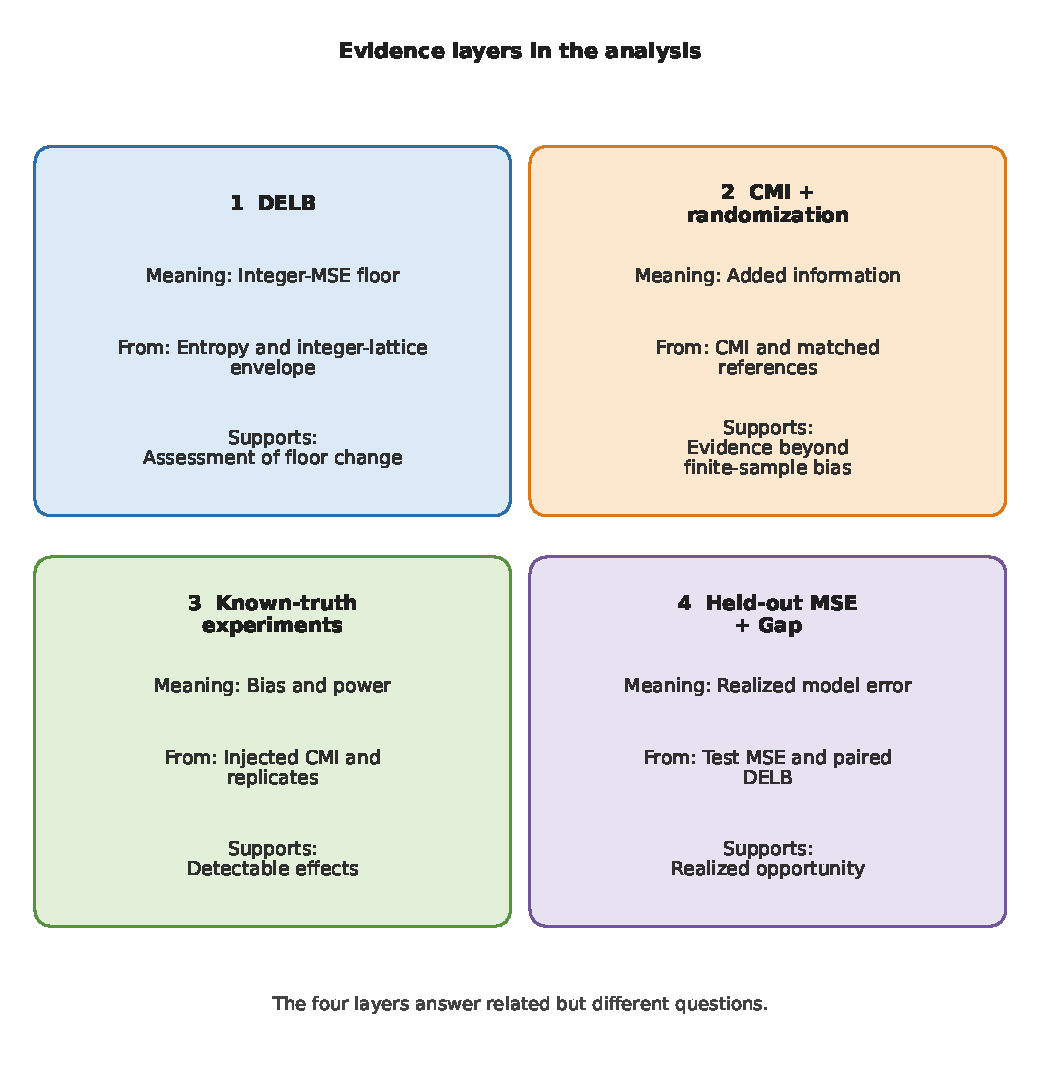
\includegraphics[width=\textwidth]{figures/problem_chain/unified_problem_chain.pdf}
\caption{Unified question-to-evidence chain. A population lower-bound
change, a calibrated finite-sample information gain, and an improvement in
realized prediction are distinct claims. CMI denotes conditional mutual
information, and DELB denotes the Discrete Entropy Lower Bound.}
\label{fig:problem_chain}
\end{figure}

Figure~\ref{fig:analysis_workflow} summarizes data processing. Crime
and bicycle records were first standardized as event-level data. They were
then aggregated to complete daily panels on a common 1~km grid. The upper
branch estimates conditional entropy, conditional mutual information (CMI),
and the DELB; the lower branch evaluates matched integer-valued
predictors. Their outputs are combined only after the information sets and
evaluation periods have been aligned.

\begin{figure}[!t]
\centering
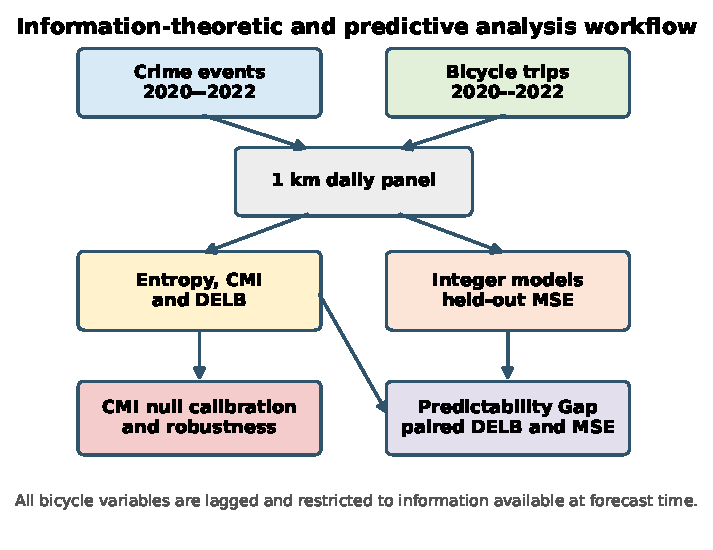
\includegraphics[width=\textwidth]{figures/e11/e11_analysis_workflow.pdf}
\caption{Data-processing and matched-analysis workflow. All
bicycle variables are lagged and restricted to information observed when
the one-day-ahead forecast is issued.}
\label{fig:analysis_workflow}
\end{figure}

\subsection{Crime Events and Cross-City Harmonization}
\label{subsec:crime_data}

The raw crime files were harmonized at the event level. We retained the
authoritative standardized field \texttt{crime\_type\_unified} and did not
reclassify it in later experiments. The analytic outcome combines three
mutually exclusive categories: property theft, vehicle theft, and burglary.
The source-category crosswalk is reported in
Appendix~\ref{app:empirical_details}. Events were assigned to their source
file's calendar year; 35 Washington, DC records whose event dates fell
outside that year were placed in a reason-coded exclusion table. Stable
event identifiers, source file hashes, source row numbers, original
categories, timestamps, and coordinates were retained for auditability.

Standardization produced 503,157 valid crime events. After applying the prespecified
spatial domain described below, \TotalCrimeEvents{} events entered the
complete analytic panels. The primary prediction target,
\(C_{c,i,t}\), is the unbinned daily count of all three harmonized
categories in city \(c\), grid cell \(i\), and local calendar day \(t\).
Category-specific counts are used only in the heterogeneity analysis.

\subsection{Bicycle Trips and Endpoint Flows}
\label{subsec:bicycle_data}

Schemas differed across the three systems and changed during the study period.
We standardized them to a common trip interface with start and end times, station identifiers,
station names, endpoint coordinates, coordinate provenance, source
identifiers, and quality-control flags. Input files were processed in
chunks, and month assignment was determined by trip start time. Blank rows
and trips assigned to a different source month were retained in
reason-coded exclusion tables. Official ride identifiers were required to
be unique after deterministic first-record retention. Exact duplicate
Vancouver records without an official unique ride identifier were retained
and flagged rather than silently removed.

Source coordinates were used when valid. Missing coordinates in Washington, DC and
New York were recovered from robust station-month medians and
temporally adjacent observations. Vancouver endpoints were matched first
to the official station identifier and then to a unique normalized station
name in the supplied official station file. Workshop, service, testing,
yard, storage, production, temporary, and valet nodes were marked
non-public. Unresolved endpoints were preserved in the standardized trip
table but were ineligible for spatial flow at that endpoint; a trip could
still contribute its other resolved public endpoint.

For each grid--day, departures and arrivals define
\(B^{\mathrm{out}}_{c,i,t}\) and \(B^{\mathrm{in}}_{c,i,t}\), with total
endpoint flow
\[
B^{\mathrm{total}}_{c,i,t}
=B^{\mathrm{out}}_{c,i,t}+B^{\mathrm{in}}_{c,i,t}.
\]
The primary mobility variable is the one-day lag of total flow. This measure captures
observable activity at both ends of a trip without including the
deterministically redundant total and net flow together with inflow and
outflow in the same entropy state. Standardization retained 87,208,600
trips; \TotalBicycleTrips{} trips had at least one flow-eligible endpoint
inside the analytic grids.

\subsection{Spatial and Temporal Panel Construction}
\label{subsec:panel_construction}

Coordinates were projected in the appropriate city coordinate reference
system and assigned to deterministic 1~km square cells anchored to the
projected coordinate-system origin. Two training-period-frozen populations
were prespecified for city-level point estimation. The complete
crime-supported domain contains every cell with at least one crime event
during 2020--2021. The bicycle-covered domain is the subset of those cells
with positive total bicycle flow during the same training period. Neither
definition uses a 2022 record. Bicycle endpoints outside the complete
crime-supported domain remained in reconciliation outputs but were not
used in either analytic population.

Every retained grid was crossed with all 1096 calendar days, including
zero-crime and zero-flow days. The resulting complete panel contains
\TotalPanelRows{} grid--day observations across 1133 cells. The
bicycle-covered panel is a fixed spatial subset of this complete panel; it
was not reconstructed from the set of nonzero-flow days. Lag construction
removed the first day of each grid only when a lagged analysis was
performed.

The temporal split was fixed before model estimation: 2020--2021 for
training, January--June 2022 for validation, and July--December 2022 for
testing. Spatial eligibility, bicycle coverage, and bicycle discretization
thresholds were determined from training records only. Model
hyperparameters were selected using training and validation data only.
The test period defined neither the domains nor any threshold, model
setting, or eligibility decision. All predictors used for a forecast were
available at issuance: no concurrent or future crime or mobility record
entered the information sets. Table~\ref{tab:variable_availability} makes
this timing explicit, and Table~\ref{tab:descriptive_statistics} summarizes
the complete panels.

\begin{table}[!htbp]
\caption{Variables, analysis units, and forecast-time availability. ``Yes,
lagged'' indicates that only information from the previous aggregation
period was used for one-period-ahead prediction.}
\label{tab:variable_availability}
\centering
\begin{tabularx}{\textwidth}{
>{\RaggedRight\arraybackslash}p{2.1cm}
>{\RaggedRight\arraybackslash}X
>{\RaggedRight\arraybackslash}p{1.7cm}
>{\RaggedRight\arraybackslash}p{1.8cm}
>{\RaggedRight\arraybackslash}p{2.0cm}}
\toprule
\textbf{Variable} & \textbf{Meaning and role} & \textbf{Spatial unit} &
\textbf{Temporal unit} & \textbf{Available at forecast time}\\
\midrule
Crime count & Daily incidents in the three harmonized crime categories;
unbinned prediction target & 1 km grid & Day & Target, no\\
Lagged crime & Previous-period crime count, discretized into four levels
(0, 1, 2, and 3+); baseline state & 1 km grid & Previous day & Yes, lagged\\
Bicycle inflow & Arrivals at resolved public endpoints; mobility primitive &
1 km grid & Previous day & Yes, lagged\\
Bicycle outflow & Departures from resolved public endpoints; mobility
primitive & 1 km grid & Previous day & Yes, lagged\\
Total bicycle flow & Sum of inflow and outflow, discretized using
training-period thresholds; added-data state & 1 km grid & Previous day &
Yes, lagged\\
Calendar state & Day of week, meteorological season, and public-holiday
status; baseline state & City/grid & Forecast day & Yes\\
Grid identifier & Fixed spatial state defined before validation and testing;
baseline state & 1 km grid & Fixed & Yes\\
\bottomrule
\end{tabularx}
\end{table}


\begin{table}[H]
\caption{Descriptive statistics for the complete 1 km grid--day panels, 2020--2022.}
\label{tab:descriptive_statistics}
\begin{adjustwidth}{-\extralength}{0cm}
\centering
\begin{tabular}{lrrrrrrr}
\toprule
\textbf{City} & \textbf{Grids} & \textbf{Grid--days} &
\textbf{Crime events} & \textbf{Bike trips} &
\textbf{Mean crime} & \textbf{Mean bike flow} & \textbf{Zero crime}\\
\midrule
Washington, DC & 186 & 203,856 & 71,397 & 7,620,562 & 0.350 & 72.95 & 77.0\%\\
New York City & 806 & 883,376 & 359,284 & 76,418,121 & 0.407 & 172.82 & 79.7\%\\
Vancouver & 141 & 154,536 & 72,447 & 2,231,293 & 0.469 & 27.37 & 75.3\%\\
\bottomrule
\end{tabular}
\end{adjustwidth}
\end{table}


Crime was sparse at the grid--day scale: zero counts represented
75.3--79.7\% of observations. New York contributed the largest system and
the highest mean daily bicycle endpoint flow, whereas Vancouver had the
highest mean property-crime count per grid--day. We report
city-specific quantities rather than treat the pooled records as exchangeable.

\subsection{Descriptive Analysis}
\label{subsec:descriptive_analysis}

Monthly and spatial summaries were computed before entropy estimation. At
the monthly level, Spearman correlations between crime and bicycle flow
were 0.505 in Washington, DC, 0.603 in New York, and 0.221 in Vancouver.
Across grids, the corresponding correlations of three-year totals were
0.637, 0.651, and 0.633. The top decile of grids accounted for 43.9, 54.3,
and 54.1\% of crime but 67.5, 89.0, and 79.7\% of bicycle flow,
respectively. These are descriptive associations and do not condition on
crime history or calendar state.

The corresponding spatial-concentration and monthly-series figures are
reported in Section S6 of the independent Supplementary Materials, so that
the main text proceeds directly to the DELB estimand and its finite-sample
validation.

\subsection{Evaluation Design Overview}
\label{sec:methods}

Analysis proceeded in the order of the research questions. We first
operationalized the target and information sets, then evaluated the
numerical DELB and examined finite-sample CMI behavior with known-truth
simulation and support diagnostics, estimated city and local point values,
calibrated them against three randomization references, and only then
compared matched held-out predictions. Fano, crime-type, and
alternative-specification analyses served as secondary checks.

\subsection{Targets and Operational Information Sets}
\label{subsec:operational_information_sets}
\label{subsec:methods_information_sets}

For the application, the generic target in Section~\ref{sec:theory} is
\begin{equation}
X_t\longmapsto C_{c,i,t}\in\mathbb Z_{\geq0},
\label{eq:crime_count_definition}
\end{equation}
the unbinned count for city \(c\), grid \(i\), and day \(t\). Bicycle
departures and arrivals are
\begin{equation}
B^{\mathrm{out}}_{c,i,t}
=\text{departures from }(c,i,t),
\qquad
B^{\mathrm{in}}_{c,i,t}
=\text{arrivals at }(c,i,t),
\label{eq:bicycle_in_out}
\end{equation}
with primitive vector
\begin{equation}
\mathbf B_{c,i,t}
=
(B^{\mathrm{out}}_{c,i,t},B^{\mathrm{in}}_{c,i,t})^\top,
\label{eq:bicycle_primitive_vector}
\end{equation}
total and net flow
\begin{align}
B^{\mathrm{total}}_{c,i,t}
&=B^{\mathrm{out}}_{c,i,t}+B^{\mathrm{in}}_{c,i,t},
\label{eq:bicycle_total_flow}\\
B^{\mathrm{net}}_{c,i,t}
&=B^{\mathrm{in}}_{c,i,t}-B^{\mathrm{out}}_{c,i,t},
\label{eq:bicycle_net_flow}
\end{align}
and lag block
\begin{equation}
\mathbf B^{(q)}_{c,i,t}
=
(\mathbf B_{c,i,t-1},\ldots,\mathbf B_{c,i,t-q}).
\label{eq:bicycle_lag_block}
\end{equation}
Total and net flow are deterministic functions of the primitive vector and
are not entered redundantly in one entropy state.

For one-day-ahead prediction, the target remained the raw nonnegative
integer count. Only conditioning variables were discretized. The previous
day's crime count was mapped to
\(\{0,1,2,\geq 3\}\). Within each city, the positive values of lagged total
bicycle flow were divided at training-period terciles; zero flow formed a
separate state. This produced four bicycle states:
\(\{\text{zero},\text{low},\text{medium},\text{high}\}\), and the fitted
cut points were reused unchanged in validation and testing.

The baseline information state was
\begin{equation}
\mathcal{S}^{0}_{c,i,t}
=\left(i,Q_C(C_{c,i,t-1}),d_t,s_t,h_t\right),
\label{eq:empirical_baseline_state}
\end{equation}
where \(d_t\), \(s_t\), and \(h_t\) denote day of week, meteorological
season, and public-holiday status. The bicycle-augmented state was
\begin{equation}
\mathcal{S}^{B}_{c,i,t}
=\left(\mathcal{S}^{0}_{c,i,t},
Q_B(B^{\mathrm{total}}_{c,i,t-1})\right).
\label{eq:empirical_bicycle_state}
\end{equation}
Only one component differs between the matched states: lagged bicycle flow.
The design excludes concurrent or future
mobility. In sigma-algebra notation,
\begin{align}
\mathcal F^0_{c,i,t}
&=\sigma(\mathcal S^0_{c,i,t}),
\label{eq:baseline_information}\\
\mathcal F^B_{c,i,t}
&=\mathcal F^0_{c,i,t}\vee
\sigma\{Q_B(\mathbf B^{(q)}_{c,i,t})\}.
\label{eq:bike_information}
\end{align}
Weather and land-use covariates were not used in the reported primary
analyses and are not claimed as controls.

\subsection{Crime-Count and Bicycle-Information Specialization}
\label{subsec:theory_application_appendix}

Using the variables defined above, the baseline entropy and bounds are
\begin{align}
H^0_{c,i,t}
&=H(C_{c,i,t}\mid\mathcal F^0_{c,i,t}),
\label{eq:crime_baseline_entropy}\\
L^0_{c,i,t}
&=\mathcal H_{\mathbb Z}^{-1}[H^0_{c,i,t}],
\label{eq:local_bound_baseline}\\
\mathbb E[(C_{c,i,t}-\widehat C_{c,i,t})^2]
&\geq L^0_{c,i,t}.
\label{eq:crime_baseline_exact_bound}
\end{align}
The closed-form counterpart is
\begin{equation}
\mathbb E[(C_{c,i,t}-\widehat C_{c,i,t})^2]
\geq
\left[\frac{2^{2H^0_{c,i,t}}}{2\pi e}-\frac1{12}\right]_+ .
\label{eq:crime_baseline_closed_bound}
\end{equation}
If \(Q_C\) top-codes the target, deterministic processing gives
\begin{equation}
H(Q_C(C)\mid\mathcal F)\leq H(C\mid\mathcal F).
\label{eq:top_coded_entropy_order}
\end{equation}

For the bicycle-augmented information set,
\begin{align}
H^B_{c,i,t}
&=H(C_{c,i,t}\mid\mathcal F^B_{c,i,t}),
\label{eq:crime_bicycle_entropy}\\
L^B_{c,i,t}
&=\mathcal H_{\mathbb Z}^{-1}[H^B_{c,i,t}],
\label{eq:local_bound_bike}
\end{align}
with the analogous closed-form bound
\begin{equation}
\mathbb E[(C_{c,i,t}-\widehat C^B_{c,i,t})^2]
\geq
\left[\frac{2^{2H^B_{c,i,t}}}{2\pi e}-\frac1{12}\right]_+ .
\label{eq:crime_bicycle_closed_bound}
\end{equation}

\begin{Proposition}[Conditional information value of bicycle mobility]
\label{prop:bicycle_information_value}
The conditional entropy reduction is
\begin{equation}
\Delta H^B_{c,i,t}
=H^0_{c,i,t}-H^B_{c,i,t}
=I(C_{c,i,t};Q_B(\mathbf B^{(q)}_{c,i,t})
\mid\mathcal F^0_{c,i,t})\geq0,
\label{eq:bicycle_information_gain}
\end{equation}
so
\begin{equation}
L^B_{c,i,t}\leq L^0_{c,i,t}.
\label{eq:bicycle_exact_bound_order}
\end{equation}
\end{Proposition}

For the discrete entropy-power shorthand
\begin{equation}
N_d(C\mid\mathcal F)=2^{2H(C\mid\mathcal F)},
\label{eq:discrete_entropy_power}
\end{equation}
\begin{equation}
\frac{N_d(C\mid\mathcal F^B)}
{N_d(C\mid\mathcal F^0)}
=2^{-2\Delta H^B}.
\label{eq:cmi_entropy_power_ratio}
\end{equation}
Finally,
\begin{equation}
I(C;Q_B(\mathbf B)\mid\mathcal F^0)
\leq I(C;\mathbf B\mid\mathcal F^0)
\label{eq:bicycle_data_processing}
\end{equation}
formalizes the information loss from binning or feature compression.


\subsection{Entropy, CMI, and Exact DELB Estimation}
\label{subsec:entropy_estimation}

For a discrete target \(C\) and state \(S\), conditional entropy was
estimated from the empirical joint probability mass function. The
Miller--Madow correction was the prespecified primary finite-sample
adjustment \citep{miller1955}; plug-in estimates were retained as diagnostic
outputs. At city level,
\begin{equation}
\widehat I^{B}_{c}
=\widehat H(C\mid\mathcal{S}^{0})
-\widehat H(C\mid\mathcal{S}^{B}).
\label{eq:empirical_cmi}
\end{equation}
Exact lower bounds were evaluated with the numerical inverse
\(\mathcal H_{\mathbb Z}^{-1}\) defined in
Equation~\eqref{eq:integer_entropy_inverse}:
\begin{equation}
\widehat L^0_c
=\mathcal H_{\mathbb Z}^{-1}
\!\left[\widehat H(C\mid\mathcal S^0)\right],
\qquad
\widehat L^B_c
=\mathcal H_{\mathbb Z}^{-1}
\!\left[\widehat H(C\mid\mathcal S^B)\right].
\label{eq:empirical_exact_bounds}
\end{equation}
The quantities of interest were
\(\widehat{\Delta L}_c=\widehat L^0_c-\widehat L^B_c\) and
\(\widehat R^L_c=\widehat{\Delta L}_c/\widehat L^0_c\).
At grid level, the corresponding population definitions are
\begin{align}
\Delta L_{c,i}
&=L^0_{c,i}-L^B_{c,i},
\label{eq:absolute_bound_reduction}\\
R^L_{c,i}
&=\frac{L^0_{c,i}-L^B_{c,i}}{L^0_{c,i}},
\qquad L^0_{c,i}>0.
\label{eq:relative_bound_reduction}
\end{align}
When sampling fluctuation made an estimated CMI negative, only its
contribution to the ordered theoretical bound was projected to zero; raw
estimates were retained in diagnostic tables. No such projection was
required for the pooled estimates reported in
Table~\ref{tab:city_entropy_results}.

Before empirical estimation, we checked the lattice partition
function, entropy--moment inversion, the zero-entropy boundary, and ordering
of exact and closed-form bounds. The validation grid covered
0--8 bits, used a lattice-tail tolerance of \(10^{-15}\), and reproduced
target discrete-Gaussian moments and entropies in simulations of up to
\(10^5\) draws.

\subsection{Sparse-State Bias and Randomization Calibration}
\label{subsec:three_inference_layers}

Three objects must be kept separate. First, the population estimand is
\(\theta=I(C;B\mid\mathcal S^0)\), which determines the ordering of the population DELB and
Fano floors after side information is added. Its finite-sample estimate can
be represented schematically as
\begin{equation}
\widehat\theta
=\theta+b(N,K_{\mathrm{obs}},S_1,\nu)+\varepsilon,
\label{eq:finite_sample_cmi_decomposition}
\end{equation}
where \(K_{\mathrm{obs}}\) is the number of observed joint atoms,
\(S_1\) is the share of observations in singleton atoms, \(\nu\) is an
effective conditional degrees of freedom, and \(\varepsilon\) denotes
sampling variation. Equation~\eqref{eq:finite_sample_cmi_decomposition} is
an organizing representation, not a claim that the bias is known from
these summaries alone.

The remaining object is the design-conditioned randomization distribution,
\(\mathcal L_\pi(\widehat\theta^\pi\mid H_0)\). Because the estimator and
state occupancy are recomputed after each transformation \(\pi\), its mean
need not equal zero. The observed statistic is compared with this reference
distribution to assess evidence under the chosen transformation, not to
validate the DELB or Fano inequalities. Figure~\ref{fig:three_layers}
summarizes the distinction.

\begin{figure}[!htbp]
\centering
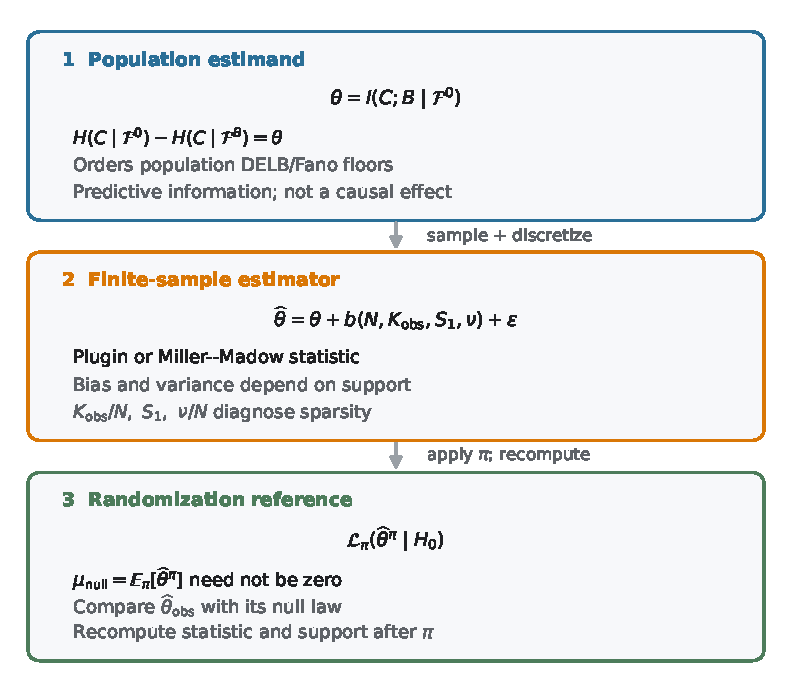
\includegraphics[width=0.92\textwidth]{figures/s7/e15_estimand_estimator_null_wide.pdf}
\caption{Population estimand, finite-sample estimator, and
transformation-specific randomization reference. CMI denotes predictive
information and is not interpreted as a causal effect.}
\label{fig:three_layers}
\end{figure}

\subsubsection{Known-Truth Sparse Nested-State Simulation}
\label{subsec:e12_simulation_methods}

Finite-sample behavior was evaluated under a fully enumerated probability
model. The baseline state \(Z\) had 4, 16, or 64 categories, the added state
\(B\) had 2, 4, or 8 categories, and the integer target followed a
negative-binomial conditional distribution. The factorial design crossed
sample sizes 365 and 1095; balanced and skewed state probabilities; zero,
moderate, and stronger population CMI; and independent or persistent Markov
state sequences. Exact summation, with the truncated tail below the
prespecified tolerance, supplied population CMI rather than treating a
large simulated sample as truth.

For each of 216 estimator cells, 150 samples were generated, yielding
32,400 replicate records. Both plug-in and Miller--Madow CMI were computed
with the same functions used in the empirical analysis, along with
\(K_{\mathrm{obs}}/N\), \(S_1\), and \(\nu/N\). A second experiment applied
the same temporal-block, spatial-series, and circular-shift transformations
to population-null and positive-CMI samples. It comprised 30 Monte Carlo
datasets per cell and 99 transformations per estimator and null design.
The reported Type I rejection rate and power assess those
specific data-generating and transformation mechanisms rather than all CMI
estimators or randomization schemes.

\subsection{DELB-Based Evaluation Algorithm}
\label{subsec:delb_evaluation_algorithm}

\begin{Algorithm}[DELB-based evaluation of an added urban data source]
\label{alg:delb_evaluation}
\textbf{Input:} integer target \(C\); baseline state \(\mathcal S^0\);
added-data state \(B\); training, validation, and test indices; entropy
estimator; randomization designs; number of repetitions \(R\).\\
\textbf{Output:} \(\widehat L^0\), \(\widehat L^B\),
\(\widehat{\Delta L}\), \(\widehat I(C;B\mid\mathcal S^0)\), support
diagnostics, randomization \(p\)-values, and matched held-out prediction
errors.
\begin{enumerate}
    \item Estimate all discretization thresholds from the training period
    and freeze them for validation and testing.
    \item Construct the baseline state \(\mathcal S^0\) and augmented state
    \(\mathcal S^B=(\mathcal S^0,B)\) on identical eligible observations.
    \item Estimate \(\widehat H(C\mid\mathcal S^0)\) and
    \(\widehat H(C\mid\mathcal S^B)\) with the same entropy estimator.
    \item Numerically evaluate
    \(\widehat L^j=\mathcal H_{\mathbb Z}^{-1}
    [\widehat H(C\mid\mathcal S^j)]\), \(j\in\{0,B\}\).
    \item Compute raw CMI, the absolute and relative estimated DELB
    reductions, and the support-density, singleton-share, and effective
    degrees-of-freedom diagnostics.
    \item For each prespecified randomization design and repetition, transform
    \(B\), reconstruct \(\mathcal S^B\), and recompute both state support and
    the complete statistic; then calculate plus-one upper-tail \(p\)-values.
    \item Fit each prediction model twice with matched samples, training
    windows, tuning rules, and all non-bicycle inputs: once with
    \(\mathcal S^0\) and once with \(\mathcal S^B\).
    \item Compare the estimated DELB change, randomization-calibrated evidence,
    and held-out MSE change as three separate outputs.
\end{enumerate}
\end{Algorithm}

\paragraph{Numerical inversion.}
For a positive entropy value, the implementation brackets the
discrete-Gaussian rate \(\lambda\) from an initial value of \(1\) by repeated
halving or doubling and then applies Brent's method. The root tolerance is
\(10^{-12}\), with at most 200 iterations. For \(\lambda\geq1\), the
partition function and second moment are evaluated by direct symmetric
integer-lattice summation. For \(\lambda<1\), the Poisson-dual theta series
avoids an unnecessarily wide real-lattice truncation. In both cases the
support radius is expanded until the analytic bound on the omitted
two-sided unnormalized tail is at most \(10^{-15}\). Entropy values at or
below zero map to a DELB of zero. Repeated resampling and randomization paths
use the configured monotone interpolation grid over 0--8 bits, with direct
inverse evaluations retained for validation.

\paragraph{Computational cost and parallelization.}
Let \(N\) be the number of matched observations, \(K_0\) and \(K_B\) the
numbers of occupied atoms in the two state tables, \(M\) the maximum retained
half-support of a lattice sum, \(T\leq200\) the number of root evaluations,
and \(J\) the number of entropy values converted to bounds. State counting
requires \(O(N)\) time and \(O(K_0+K_B)\) memory; direct bound conversion
requires \(O(JTM)\) time and \(O(M)\) additional memory. With \(R\)
randomizations, the serial calibration cost is
\(O(RN+RJTM)\), excluding model fitting, whose cost depends on the selected
predictor. Randomizations are independent conditional on their stored seeds.
The implementation evaluates city--spatial-scale--temporal-scale cells
independently and records cell-level results and seeds for reproducibility.


\subsection{City and Local DELB Estimation}
\label{subsec:city_local_information}

City-level DELB point estimates were evaluated in both training-period-frozen
populations and separately by year. The complete crime-supported domain
represents the full prespecified target population, whereas the
bicycle-covered domain represents the service-covered population in which
the added mobility channel is observed. Both sets of cells were determined
from 2020--2021 records and then applied unchanged to validation and
testing; no 2022 outcome was used to redefine either spatial population.
Their comparison therefore concerns the target analysis population rather
than an administratively fixed city boundary.

Uncertainty was evaluated with 1000 shared non-overlapping seven-day
calendar-block resamples. Resampling an entire city-day block preserved
contemporaneous dependence among grids. Reported 95\% intervals were
centered bootstrap intervals. The co-primary population designation is
limited to the city-level point-estimate comparison. Local estimation,
randomization calibration, held-out prediction, and multiscale analyses
retain their prespecified bicycle-covered domains because complete-domain
counterparts were not generated for all of those experiments.

The calculation was repeated within each grid after removing the grid
identifier from the local state. Eligibility required 1095 valid lagged
days, at least 30 crimes, at least 55 positive-flow days, no zero-flow run
longer than 365 days, and at least two observed target and bicycle states.
This yielded \TotalEligibleLocalGrids{} eligible cells. A one-sided
normal screen based on the seven-day block bootstrap was adjusted by the
Benjamini--Hochberg procedure \citep{benjamini1995}; because state-space
sparsity can bias entropy differences, it is described as a
\emph{sampling-uncertainty screen}, not as a randomization test of
conditional independence. Spatial clustering was summarized with global
and local Moran statistics \citep{moran1950} using row-standardized queen
contiguity and 999 permutations.

\subsection{Three-Axis Scale and Sample-Size Design}
\label{subsec:e16_scale_methods}

To distinguish changes in the prediction target from changes in estimator
stability, the multiscale design crossed three spatial resolutions (500~m,
1~km, and 2~km),
two temporal resolutions (day and complete ISO week), and five sample
fractions (20, 40, 60, 80, and 100\%). The comparison domain comprised
complete 2~km parents, their four 1~km children, and all sixteen 500~m
descendants. Crime and bicycle totals reconciled exactly across this nested
common footprint. Weekly records were sums over seven complete days, and a
one-period lag always referred to the preceding aggregation period.

Sample fractions were formed by retaining all grids in selected time blocks.
Daily panels used complete seven-day blocks and weekly panels used complete
four-week blocks, stratified by year and season. Fractions were nested within
each of 50 frozen repetitions; a separate five-point expanding-window design
diagnosed chronological accumulation and possible distribution drift.
Estimator stability was measured by
\begin{equation}
S_N(\widehat\theta)
=\frac{|\widehat\theta_N-\widehat\theta_{N_{\max}}|}
{\max(|\widehat\theta_{N_{\max}}|,10^{-12})},
\label{eq:e16_stability}
\end{equation}
where \(\widehat\theta\) denotes an estimated entropy, CMI, or DELB quantity.
It measures convergence to the full-sample estimate, not error relative to
unknown population truth.

Count-level DELBs remained primary. For a square-cell area \(A\) in km\(^2\)
and aggregation duration \(\tau\) in days, the deterministically scaled crime
intensity target has
\begin{equation}
L_{\mathrm{int,MSE}}^{j}(A,\tau)
=\frac{L^{j}(A,\tau)}{(A\tau)^2},
\qquad
L_{\mathrm{int,RMSE}}^{j}(A,\tau)
=\frac{\sqrt{L^{j}(A,\tau)}}{A\tau},
\quad j\in\{0,B\}.
\label{eq:e16_intensity_normalization}
\end{equation}
The transformation applies to the correspondingly scaled count target; it
does not make daily and weekly targets, or different spatial aggregates, the
same estimand. No DELB or CMI was divided by sample size.

Randomization calibration covered all 90 city--space--time--sample cells.
Each cell used 199 temporal-block, spatial-series, and circular-shift
replicates; the prespecified 500~m--day, 1~km--day, and 2~km--week scales used
999 replicates. Fractions below 100\% used the lowest-index frozen thinning
path (replicate 1), whereas the stability analysis separately summarized all
50 thinning paths. Temporal blocks contained seven days or four weeks;
circular shifts were separated by at least 31 days or five weeks.
Miller--Madow CMI, DELB reduction, support atoms, singleton share, and
effective degrees of freedom were recomputed after every transformation.
Plus-one upper-tail \(p\)-values were adjusted both across all 270 tests and
within city--null-design families. These are design-conditioned diagnostics
rather than exact conditional randomization tests.

\subsection{Matched Prediction and Predictability Gap}
\label{subsec:prediction_experiment}
\label{subsec:methods_prediction}

Four model families were compared under the paired states in
Equations~\eqref{eq:empirical_baseline_state} and
\eqref{eq:empirical_bicycle_state}: a smoothed state mean, a Poisson
generalized linear model (GLM), a negative-binomial GLM, and histogram
gradient boosting with Poisson loss. Within each family, baseline and
bicycle-aware specifications used the same target, sample, preprocessing,
training period, tuning rule, and integer post-processing. The bicycle-aware
version added only \(Q_B(B^{\mathrm{total}}_{t-1})\). A seven-day seasonal
naive predictor was retained as an external descriptive benchmark but was
not matched to the DELB state and was not used in the principal comparisons.

Hyperparameters were selected by validation-period integer MSE. Continuous
nonnegative predictions were converted to integer counts using half-up
rounding. The primary metric was
\begin{equation}
\operatorname{MSE}^{j}_{c,k}
=\frac{1}{N_c}\sum_{(i,t)\in\mathcal T_c}
\left(C_{c,i,t}-\widehat C^{\,j}_{c,i,t,k}\right)^2,
\quad j\in\{0,B\},
\label{eq:empirical_mse}
\end{equation}
where \(k\) indexes the model family and \(\mathcal T_c\) is the fixed
July--December 2022 test set. Positive
\(\Delta\operatorname{MSE}_{c,k}
=\operatorname{MSE}^{0}_{c,k}-\operatorname{MSE}^{B}_{c,k}\)
denotes improvement. One thousand shared non-overlapping seven-day test
blocks preserved cross-grid dependence. Family-level screens used
one-sided normal approximations and Benjamini--Hochberg adjustment.

\subsection{Secondary Fano, Heterogeneity, and Robustness Designs}
\label{subsec:fano_validation_methods}

Fixed finite-label targets complemented the integer-count MSE analysis. The
primary target was
\[
Y^{(2)}_{c,i,t}=\mathbf 1\{C_{c,i,t}>0\},
\]
and the robustness target mapped \(C=0\), \(C=1\), and \(C\geq2\) to three
classes. These thresholds were fixed globally and were not selected from
city or test outcomes. Baseline and bicycle-augmented states were exactly those
in Equations~\eqref{eq:empirical_baseline_state} and
\eqref{eq:empirical_bicycle_state}.

Conditional entropy and the Fano floor were estimated on the combined
training and validation period. A statewise modal classifier was then
evaluated on the unchanged July--December 2022 test period. Test states
unseen before July 2022 used the pretest global mode; no test label was used
to set a fallback. Uncertainty used 300 non-overlapping seven-day
calendar-block bootstrap samples. Centered intervals were reported because
unconditional resampling can itself remove rare states; the raw bootstrap
means were retained as diagnostics.

An oracle check reused the enumerated simulation models and compared the
true Bayes error with the true Fano floor for binary and three-level targets.
The empirical comparison contrasted an estimated pretest floor with a held-out
classifier error. Estimated violations, if present, were retained as
finite-sample or distribution-shift diagnostics. DELB and Fano values were
never numerically compared because their targets and losses differ.

\subsubsection{Predictability Gap and Theory--Practice Comparison}
\label{subsec:gap_methods}
\label{subsec:gap_efficiency}

The model-specific predictability gap was
\begin{equation}
G^j_{c,k}=\operatorname{MSE}^{j}_{c,k}-L^j_c
\label{eq:empirical_gap}
\end{equation}
and its narrowing,
\begin{equation}
\Delta G_{c,k}
=G^0_{c,k}-G^B_{c,k}
=\Delta\operatorname{MSE}_{c,k}-\Delta L_c.
\label{eq:empirical_gap_narrowing}
\end{equation}
In population notation, the same accounting quantity is
\begin{equation}
G=\operatorname{MSE}-L,
\label{eq:prediction_gap}
\end{equation}
and an information-use ratio may be reported only when its denominator is
positive:
\begin{equation}
\eta=\frac{\Delta\operatorname{MSE}}{\Delta L}.
\label{eq:bound_efficiency}
\end{equation}
A positive \(\Delta G\) means that empirical error fell by more than the
estimated floor; a negative value means that the theoretical opportunity
expanded faster than the tested model used it. For the test comparison,
the exact bounds were re-estimated on the matched test-window information
states.

At the local scale, pretest \(\Delta L_{c,i}\) from training plus
validation was compared with test-period
\(\Delta\operatorname{MSE}_{c,i,k}\). Spearman correlations used 2000
paired-grid bootstrap resamples and false-discovery-rate adjustment.
Separate ordinary least-squares models regressed local empirical
improvement on local theoretical reduction with city fixed effects and
HC3 standard errors. These analyses are descriptive: cross-grid dependence
was not modeled in the regression covariance.

\subsubsection{Crime-Type Heterogeneity}
\label{subsec:crime_type_methods}

The information and matched-prediction analyses were repeated for property
theft, vehicle theft, and burglary, using category-specific lagged counts
but the same bicycle thresholds and temporal split. This produced 18
city--category theory estimates (pooled and test), 36 paired test prediction
contrasts, and paired within-city category comparisons. Seven-day block
resampling and Benjamini--Hochberg adjustment were applied as in the primary
experiments.

\subsubsection{Alternative Specifications and Null Calibration}
\label{subsec:robustness_null_methods}

Prespecified robustness analyses examined whether the sign of the estimated
DELB reduction persisted across design changes. The 16 theory
specifications comprised
500~m, 1~km, and 2~km grids; daily and weekly targets; alternative crime and
bicycle state mappings; crime and bicycle lags through seven days; and
inflow, outflow, and absolute net flow. Each specification was estimated
with plug-in, Miller--Madow, and a coherent Jeffreys--Dirichlet estimator.
For the latter, a single symmetric Dirichlet posterior was placed on the
observed atoms of \((C_t,\mathcal S^0_t,B_{t-1})\), and both conditional
entropies were obtained by marginal aggregation of that posterior. Bootstrap
intervals were recomputed with 7-, 14-, and 28-day blocks. Predictive
stability was assessed at 12 expanding monthly origins in 2022, each with a
one-month evaluation window and the same four model families.

Three diagnostics assessed whether the observed CMI exceeded finite-sample
reference distributions. A temporal-block permutation reassigned seven-day mobility
blocks, a spatial-series permutation reassigned entire mobility histories
among grids, and a circular-shift surrogate displaced each grid's mobility
series by an admissible random offset. Each design used 999 transformations,
upper-tail randomization \(p\)-values, and Benjamini--Hochberg correction.
The same designs were applied to the 339 eligible grids. A local cell
was declared null-calibrated only if it passed all three adjusted tests.
Finally, matched 14- and 30-day mobility lags were compared with the recent
one-day lag. These procedures are diagnostic randomization tests, not exact
conditional randomization tests and not tests of a causal bicycle effect.

E17 assessed whether the city-level calibration depended on the primary
Miller--Madow correction. On each of the identical E10 surrogates, it
recomputed plug-in, Miller--Madow, and coherent observed-support
Jeffreys--Dirichlet CMI. Plus-one upper-tail \(p\)-values were adjusted in
two prespecified families: nine city--design comparisons within each
estimator and all 27 estimator--city--design comparisons globally. E17 did
not rerun the 339-cell local screen. The Jeffreys calculation regularizes
the probabilities of observed full-joint atoms; it does not impute
unobserved support.

E18 added a baseline-state-matched restricted randomization at the city
level. Each grid series was partitioned into complete seven-day blocks.
Blocks were permuted without replacement within grid, year, and season
after ordering them by the distribution of lagged-crime states and holiday
occupancy; strata with fewer than five blocks were widened within year.
Terminal incomplete blocks remained fixed. The design used 999
randomizations, plus-one upper-tail \(p\)-values, and a three-city
Benjamini--Hochberg family. Prespecified diagnostics required at least 80\%
of blocks to be movable and an absolute standardized difference no larger
than 0.10 for the bicycle-state marginal.

A semi-synthetic experiment evaluated calibration and power on fixed
empirical state supports. Six flow-quantile-spanning grids and 365 days
were selected deterministically per city. Negative-binomial targets were
generated from shrinkage estimates depending only on the baseline state
under the null; centered bicycle-state effects were then calibrated by
enumeration to target population CMI values of 0, 0.02, 0.05, and 0.10
bit, subject to the maximum attainable value on each support. The factorial
design crossed three cities, fitted and enhanced-overdispersion scenarios,
and the original temporal-block and restricted matched-block references.
Each cell used 50 Monte Carlo datasets and 99 randomizations. Exact
binomial 95\% intervals accompanied Type I error and power. This restricted
design is closer to the baseline state than E10, but it is not an exact
conditional randomization test because it does not sample from a known
\(B\mid\mathcal S^0\) distribution.

\subsubsection{Surrogate-Specific Support Diagnostics}
\label{subsec:e13_support_methods}

Each accepted surrogate was reconstructed from its original seed, after which
both CMI and state support were recomputed. For each observed or randomized
sample, the recorded quantities were
\begin{equation}
K_{\mathrm{obs}}
=\#\{(C,Z,B)\text{ observed atoms}\},
\qquad
S_1
=\frac{\#\{\text{observations in singleton atoms}\}}{N},
\label{eq:e13_support_metrics}
\end{equation}
and
\begin{equation}
\nu=\sum_z(r_z-1)(c_z-1),
\label{eq:e13_effective_df}
\end{equation}
where \(r_z\) and \(c_z\) are the observed target and bicycle-state
cardinalities within baseline state \(z\). The analysis used
\(K_{\mathrm{obs}}/N\), \(S_1\), and \(\nu/N\).

Simulation-based associations related null bias to these support
metrics. Empirical associations were reported descriptively with
Spearman correlations and city and null-design fixed-effects regressions
using city-grid-clustered standard errors. Models related the null mean to
mean surrogate support and observed-minus-null CMI to surrogate-minus-
observed support change. These associations diagnose a finite-support
mechanism; they do not turn the null mean into an estimator-bias estimate or
identify a causal effect.

\subsection{Reproducibility and Analysis Scope}
\label{subsec:reproducibility}

Every experiment was executed through a Python entry point configured by a
versioned YAML file. Run directories contain environment
snapshots, random seeds, source-run pointers, row reconciliations, acceptance
checks, machine-readable tables, diagnostic workbooks, and figures. All
manuscript figures were generated by the corresponding Python experiment;
none was manually edited. E11 reads only accepted E02 and E04--E10 outputs,
while the S7 Python synthesis reads accepted E12--E15 outputs and copies a
hash-verified figure set into the manuscript. E09 and E10 were frozen before
output inspection; E12--E14 retain replicate-level simulation, support, and
bootstrap records; E15 retains both single- and double-column vector
versions of the conceptual figure. All accepted outputs remain in the
versioned run lineage. E16 similarly reads only accepted multiscale panels,
sample indices, estimates, and randomization outputs; its S16.7 Python
synthesis generates the LaTeX macros and tables and copies all scale figures
after SHA-256 verification. A minimal known-truth example at
\texttt{examples/minimal\_delb\_cmi\_simulation.py} reproduces the population
CMI ordering and discrete-envelope DELB inversion without city data; it is pedagogical and
does not replace the registered E12 simulation grid.

\section{Results}
\label{sec:results}

The results begin with the multicity application outcome and then unpack
the evidence needed to interpret it. After the application overview, we
examine finite-sample behavior under known population conditions, report
the detailed city-level and local DELB estimates, evaluate them against
prespecified randomization references, assess sensitivity to spatial scale,
temporal aggregation, and sample size, and compare the estimated bounds
with held-out prediction errors. Table~\ref{tab:results_evidence_map}
summarizes the question addressed by each evidence layer.
Throughout this section, estimated CMI, changes in the estimated DELB,
randomization-calibrated information gain, and changes in realized
prediction error are treated as distinct empirical quantities.

\begin{table}[!t]
\begin{adjustwidth}{-\extralength}{0cm}
\caption{Evidence map for interpreting the empirical results. CMI denotes
conditional mutual information, and DELB denotes the Discrete Entropy Lower
Bound.}
\label{tab:results_evidence_map}
\scriptsize
\begin{tabularx}{\fulllength}{p{0.14\fulllength}XXX}
\toprule
\textbf{Evidence layer} & \textbf{Question answered} & \textbf{Main result} & \textbf{Interpretive boundary} \\
\midrule
City and local point estimates &
Does the estimated prediction floor decline after the bicycle state is added? &
Estimated conditional entropy and the corresponding DELB declined in all
cities and in the reported local summaries. &
Describes an estimated state-partition difference; it does not establish
bicycle-specific information. \\
Known-truth simulation and support diagnostics &
Can positive estimated CMI arise when population CMI is zero? &
Sparse nested states produced positive plug-in and Miller--Madow estimates
and nonzero randomization centers; support complexity tracked both behaviors. &
Diagnoses finite-sample estimation and calibration, not the city-specific
mobility effect. \\
Randomization and multiscale calibration &
Is the observed statistic unusually large under prespecified null mechanisms? &
No primary or multiscale comparison survived the relevant calibration and
multiplicity correction. &
Limits attribution to recent, geographically matched bicycle mobility; it
does not prove conditional independence. \\
Matched prediction and Predictability Gap &
Did fitted models convert the augmented state into lower held-out MSE? &
Improvements were model- and city-dependent, and only two New York models
narrowed the estimated gap. &
Realized model performance neither proves nor refutes a population DELB
change. \\
Fano comparison &
Does the information ordering persist under classification loss? &
Estimated Fano floors declined, while sparse held-out modal classifiers often
worsened. &
Fano and DELB use different targets and losses; their magnitudes are not
directly comparable. \\
Heterogeneity and robustness &
Does the descriptive pattern depend on target or specification? &
Positive DELB-reduction point estimates were widespread, whereas predictive
improvements remained heterogeneous. &
Changed targets and units preclude direct effect-size comparisons; category
results are exploratory. \\
\bottomrule
\end{tabularx}
\end{adjustwidth}
\end{table}

\subsection{Multicity Application Results at a Glance}
\label{subsec:application_results_overview}

\begin{table}[!htbp]
\caption{Application-level synthesis across the three cities. The
transformation-reference column reports the smallest unadjusted \(p\)-value
across the temporal-block, spatial-series, and circular-shift references; the
matched-reference column reports the \(p\)-value from baseline-state-matched
restricted randomization. Positive prediction screens are adjusted within
the matched city--model comparisons.}
\label{tab:application_results_overview}
\centering
\setlength{\tabcolsep}{2pt}
\begin{tabular*}{\textwidth}{@{\extracolsep{\fill}}lrrrrrr@{}}
\toprule
\textbf{City} & \shortstack{\textbf{Complete-domain}\\\(\boldsymbol{\Delta L}\)} &
\shortstack{\textbf{Covered}\\\(\boldsymbol{\Delta L}\)} &
\shortstack{\textbf{Covered relative}\\\textbf{reduction}} &
\shortstack{\textbf{Transform.}\\\textbf{min. \(p\)}} &
\shortstack{\textbf{Matched}\\\(\boldsymbol{p}\)} &
\shortstack{\textbf{Positive screens /}\\\textbf{gap narrowing}}\\
\midrule
Washington, DC & 0.0119 & 0.0123 & 7.9\% & 0.967 & 0.599 & 0/4 \quad / \quad 0/4\\
New York City & 0.0094 & 0.0604 & 17.3\% & 0.986 & 0.999 & 2/4 \quad / \quad 2/4\\
Vancouver & 0.0115 & 0.0919 & 18.0\% & 0.903 & 0.994 & 1/4 \quad / \quad 0/4\\
\bottomrule
\end{tabular*}
\end{table}


The application produced a consistent descriptive ordering but not a
consistent inferential or predictive gain
(Table~\ref{tab:application_results_overview}). Within the
bicycle-covered populations, adding lagged bicycle flow reduced the
estimated DELB by 7.9\% in Washington, DC, 17.3\% in New York City, and
18.0\% in Vancouver. The reductions remained positive in the complete
crime-supported populations, although they attenuated sharply in New York
City and Vancouver.

Neither the three E10 transformation references nor the E18
baseline-state-matched reference separated the observed CMI in any city.
Held-out prediction was also selective: adjusted positive-improvement
screens occurred for two of four New York models and one Vancouver model,
whereas only the two New York models narrowed the estimated Predictability
Gap. Thus, the direct application result is not that bicycle mobility
uniformly improves crime prediction. It is that a positive estimated
information-floor change can coexist with non-rejection under calibrated
references and model-dependent realized performance. The following
subsections provide the finite-sample and experiment-specific evidence
behind that synthesis.

\subsection{Finite-Sample Behavior of CMI Estimation}
\label{subsec:results_e12_simulation}

Known-truth simulations were examined before the urban estimates to
determine how sparse nested states affect CMI estimation and
transformation-based calibration. Population CMI was obtained
by exact enumeration, so estimator bias could be separated from the
center of the corresponding randomization distribution.

Under the 72 population-null design cells, both estimators produced
positive CMI estimates despite the true CMI being zero. Mean null bias
was \SimPluginNullBias{} bits for the plug-in estimator and \SimMMNullBias{} bits
for the Miller--Madow estimator. Increasing the sample size from 365 to 1095
observations reduced average bias, whereas larger joint state spaces,
greater singleton occupancy, and larger effective conditional degrees
of freedom increased it. The Miller--Madow correction reduced average
bias but did not uniformly outperform the plug-in estimator in the
sparsest designs.

The transformation-specific reference distributions were also positively centered.
Their mean centers were \SimPluginNullCenter{} bits for the plug-in estimator
and \SimMMNullCenter{} bits for the Miller--Madow estimator. Despite these nonzero centers,
the mean Type I rejection rates were \SimPluginTypeI{} and \SimMMTypeI{},
respectively, because the observed statistics were compared with their
complete transformation-specific reference distributions rather than with
zero. Mean power across the positive-CMI designs was \SimPluginPower{} for
the plug-in estimator and \SimMMPower{} for the Miller--Madow estimator (Table~\ref{tab:e12_simulation_summary}
and Figure~\ref{fig:e12_sparse_simulation}).

\begin{table}[!htbp]
\caption{Finite-sample CMI simulation summary. Null bias and null centers are in bits. Size is the mean rejection rate under population CMI equal to zero; power averages the positive-CMI designs.}
\label{tab:e12_simulation_summary}
\centering
\begin{tabular*}{\textwidth}{@{\extracolsep{\fill}}lcccc@{}}
\toprule
\textbf{Estimator} & \textbf{Mean null bias} & \textbf{Mean null center} & \textbf{Size} & \textbf{Power}\\
\midrule
Plug-in & 0.1651 & 0.2069 & 0.014 & 0.337\\
Miller--Madow & 0.1264 & 0.1376 & 0.011 & 0.447\\
\bottomrule
\end{tabular*}
\end{table}


\begin{figure}[H]
\begin{adjustwidth}{-\extralength}{0cm}
\centering
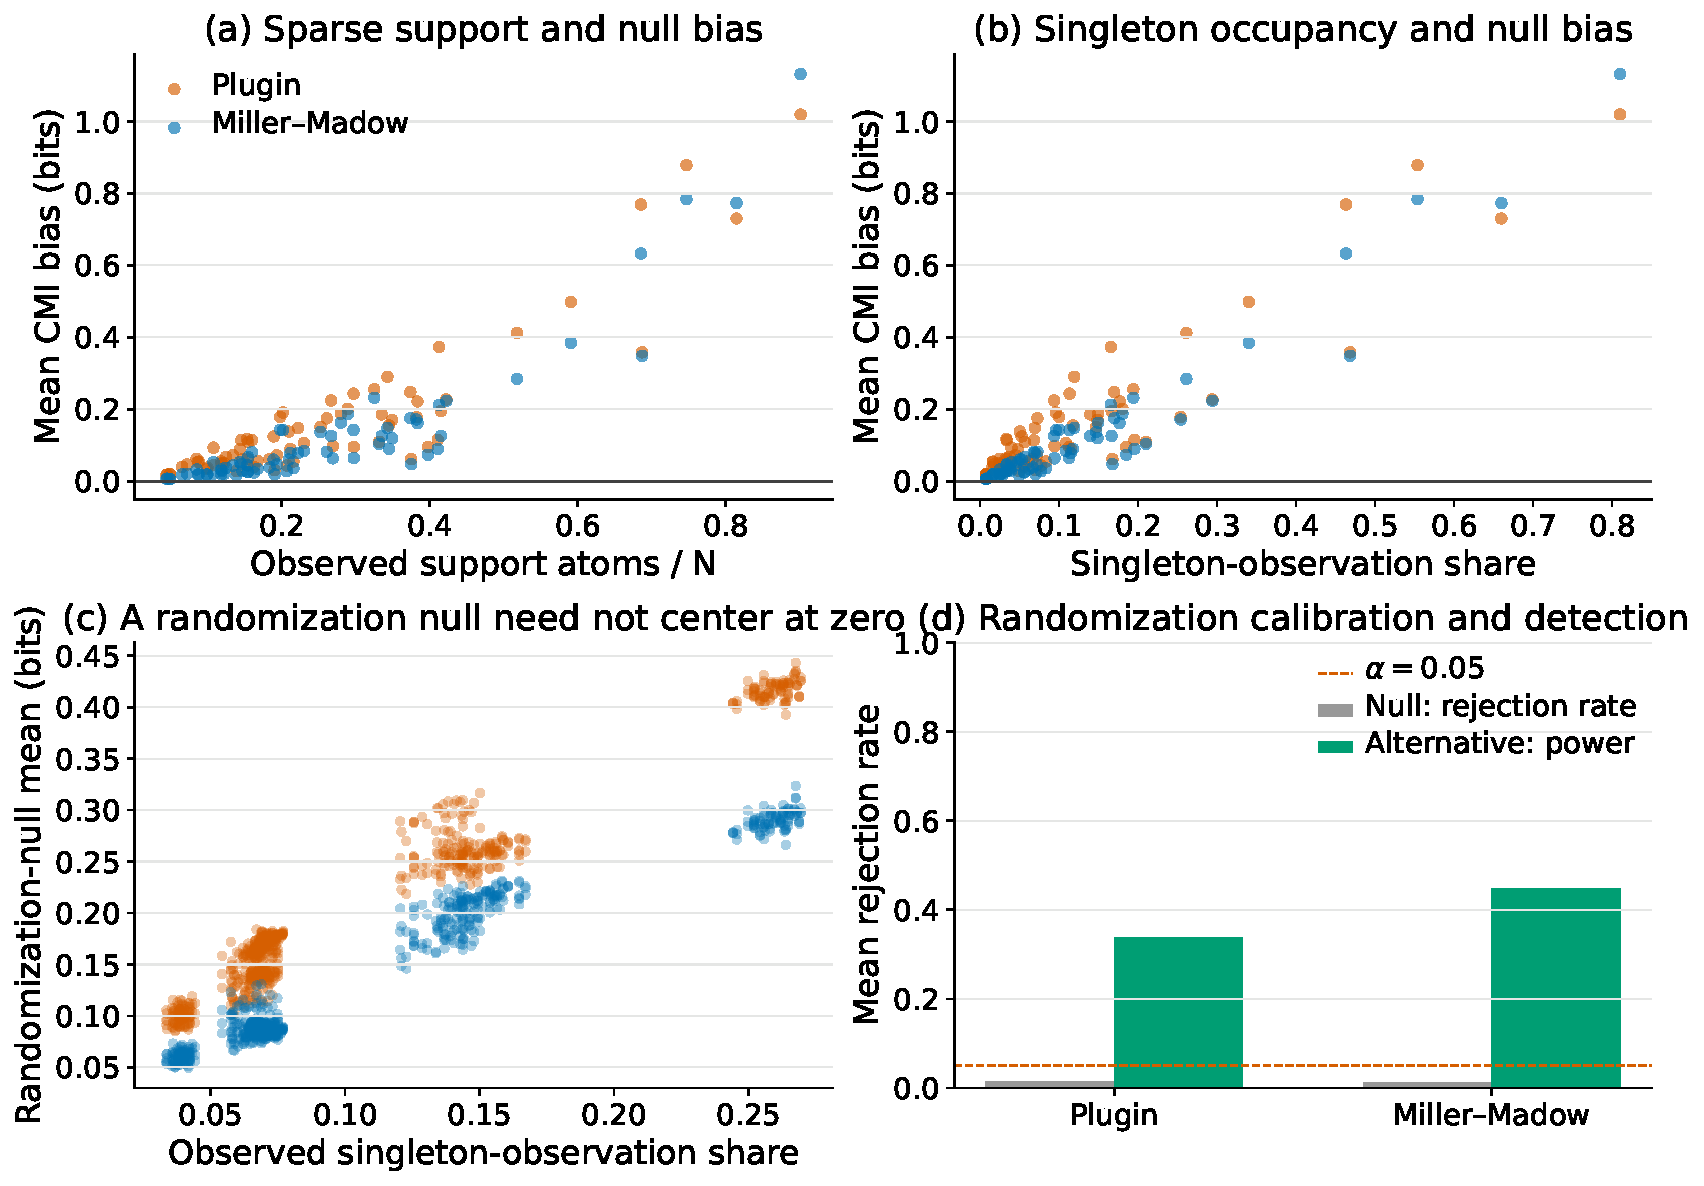
\includegraphics[width=\linewidth]{figures/s7/e12_sparse_cmi_main.pdf}
\end{adjustwidth}
\caption{Known-truth simulation of sparse nested-state CMI estimation and
randomization behavior. Population CMI is obtained by exact enumeration.
Positive estimator bias and a positive randomization center are distinct
finite-sample objects.}
\label{fig:e12_sparse_simulation}
\end{figure}

Support diagnostics showed consistent associations with finite-sample
behavior. In the known-null simulations, observed-atom density,
singleton-observation share, and normalized effective degrees of freedom
were associated with the bias of both estimators. Across the 1017 empirical
city--grid--reference summaries, their Spearman correlations with the
randomization-reference mean were 0.835, 0.866, and 0.988, respectively.
In a fixed-effects model with city-grid-clustered standard errors,
surrogate normalized effective degrees of freedom had a coefficient of
\SupportCombinedNuCoefficient{} (SE \SupportCombinedNuSE{};
\(R^2=\SupportCombinedNullRSquared{}\)).

The transformations also changed the CMI support.
Changes in support complexity between each surrogate and the observed
table were negatively associated with observed-minus-reference CMI, with correlations ranging
from \(-0.653\) to \(-0.791\). These relations are diagnostic rather than
causal and do not define a universal bias correction. They show that the
center of a finite-sample randomization distribution depends jointly on
the estimator, observed support, and transformation design. Accordingly,
the city analyses below compare observed CMI with complete design-matched
reference distributions rather than using zero as an automatic benchmark.



\begin{table}[H]
\caption{Association of support diagnostics with CMI estimator behavior. Entries are Spearman correlations. The first two columns use population-null simulations; the last two use 1,017 city-grid-null summaries.}
\label{tab:e13_support_relationships}
\begin{adjustwidth}{-\extralength}{0cm}
\centering
\small
\begin{tabular}{lrrrr}
\toprule
\textbf{Metric} & \textbf{Plugin bias} & \textbf{MM bias} & \textbf{Null mean} & \textbf{Observed--null}\\
\midrule
$K_{\mathrm{obs}}/N$ & 0.840 & 0.891 & 0.835 & -0.653\\
$S_1$ & 0.819 & 0.909 & 0.866 & -0.656\\
$\nu/N$ & 0.989 & 0.950 & 0.988 & -0.791\\
\bottomrule
\end{tabular}
\end{adjustwidth}
\end{table}


\begin{figure}[H]
\begin{adjustwidth}{-\extralength}{0cm}
\centering
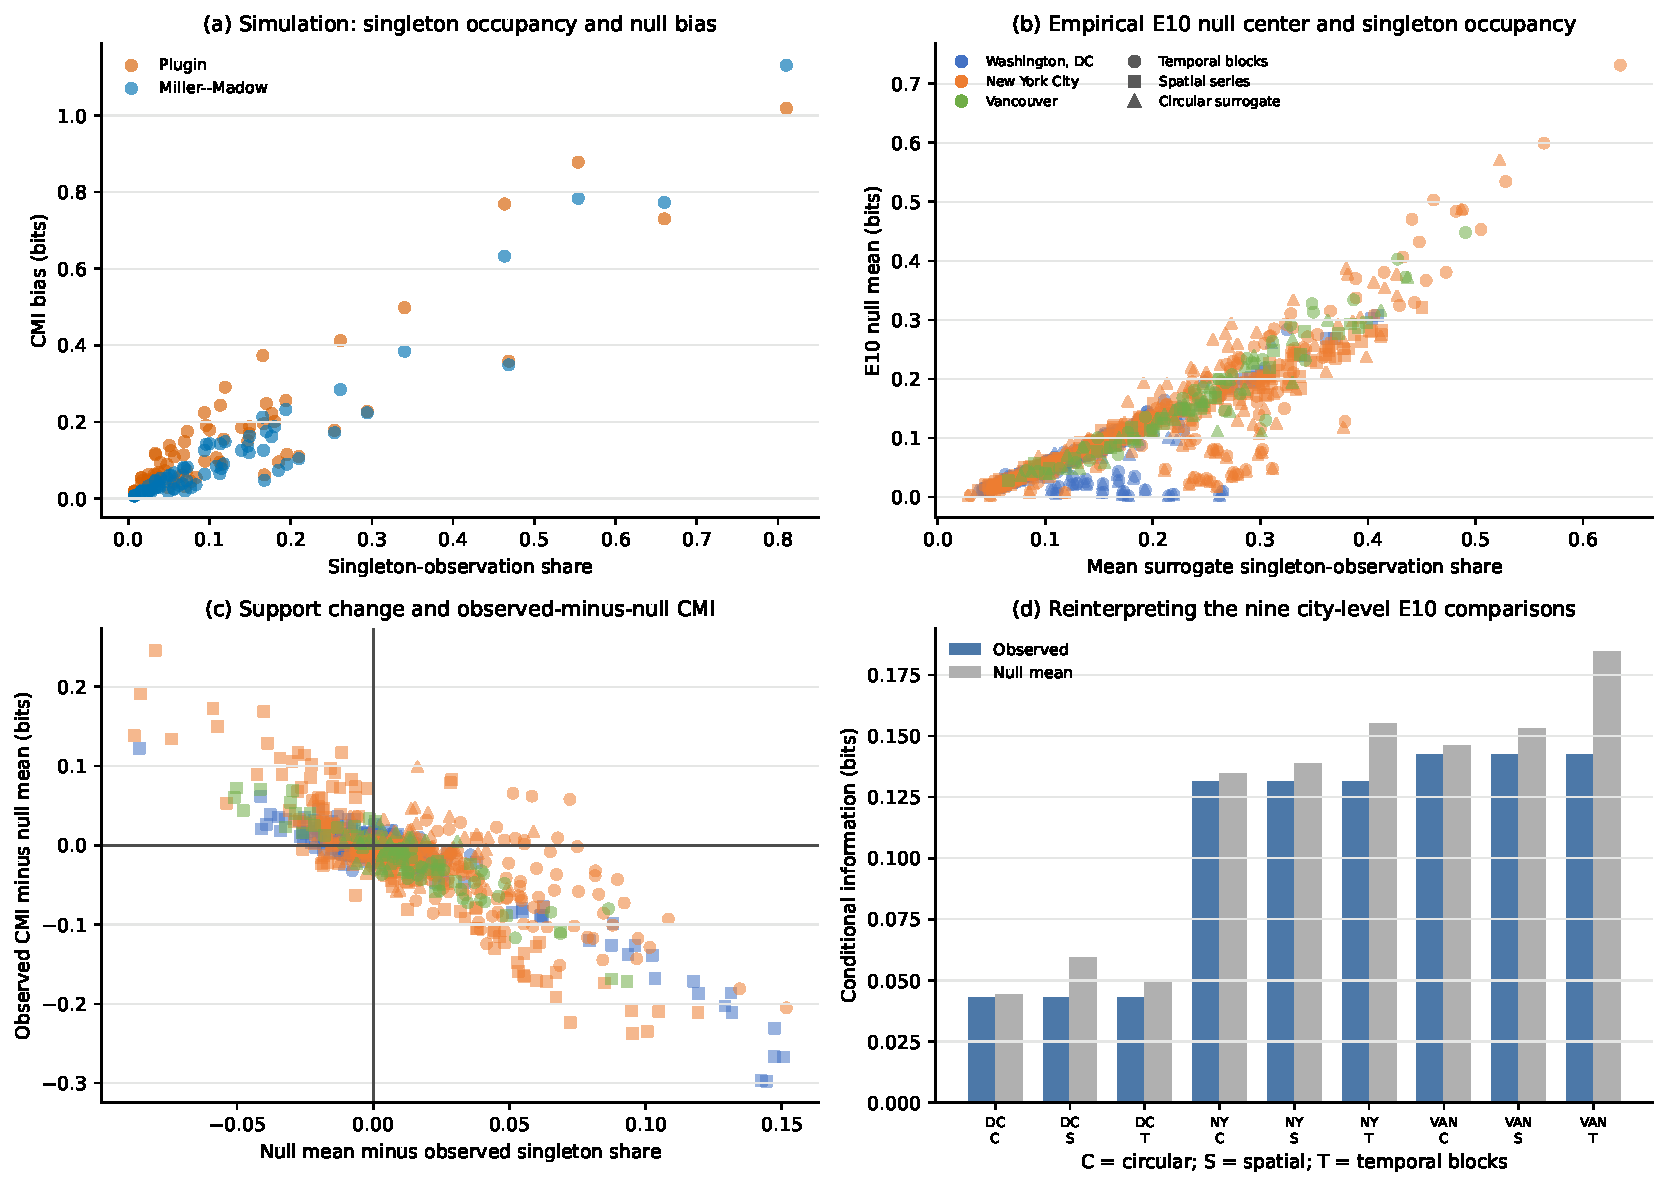
\includegraphics[width=\linewidth]{figures/s7/e13_support_null_main.pdf}
\end{adjustwidth}
\caption{Support structure and randomization-reference centering. Simulation
panels use known zero population CMI; empirical panels use
surrogate-specific support recomputed after every transformation. Lines are
descriptive associations.}
\label{fig:e13_support_null}
\end{figure}

\subsection{Estimated City-Level and Local Prediction Bounds}
\label{subsec:results_city_information}

At the pooled city level, adding the one-day-lagged bicycle state reduced
estimated conditional entropy in all three cities. The Miller--Madow CMI
estimates were \DCCMI{} bits in Washington, DC,\NYCMI{} bits in New York, and \VANCMI{} bits in Vancouver.
Mapping the baseline and bicycle-augmented conditional entropies through the
same inverse integer-lattice envelope produced estimated DELB reductions of
\DCDeltaL{} MSE units in Washington, DC, \NYDeltaL{} in New York City, and
\VANDeltaL{} in Vancouver. These changes represented relative reductions of
\DCRelativeL, \NYRelativeL, and \VANRelativeL, respectively
(Table~\ref{tab:city_entropy_results} and
Figure~\ref{fig:city_information_bounds}).
The centered seven-day block-bootstrap intervals for the CMI estimates
excluded zero. These intervals quantify sampling variation under the
observed state partition and dependence structure; randomization-based
attribution is examined separately in Section~\ref{subsec:results_nulls}.



\begin{table}[H]
\caption{Pooled city-level conditional entropy and DELB results in the training bicycle-covered domain. Brackets report centered 95\% seven-day block-bootstrap intervals for CMI.}
\label{tab:city_entropy_results}
\begin{adjustwidth}{-\extralength}{0cm}
\centering
\begin{tabular*}{\linewidth}{@{\extracolsep{\fill}}lrrrrrrrr@{}}
\toprule
\textbf{City} & \(\boldsymbol{N}\) & \(\boldsymbol{H^0}\) &
\(\boldsymbol{H^B}\) & \textbf{CMI [95\% CI]} &
\(\boldsymbol{L^0}\) & \(\boldsymbol{L^B}\) &
\(\boldsymbol{\Delta L}\) & \(\boldsymbol{R^L}\)\\
\midrule
Washington, DC & 198,195 & 0.783 & 0.740 & 0.043 [0.040, 0.047] & 0.157 & 0.144 & 0.012 & 7.9\%\\
New York City & 216,810 & 1.293 & 1.162 & 0.131 [0.123, 0.140] & 0.350 & 0.290 & 0.060 & 17.3\%\\
Vancouver & 37,230 & 1.563 & 1.421 & 0.142 [0.126, 0.159] & 0.511 & 0.419 & 0.092 & 18.0\%\\
\bottomrule
\end{tabular*}
\end{adjustwidth}
\end{table}


\begin{figure}[!t]
\centering
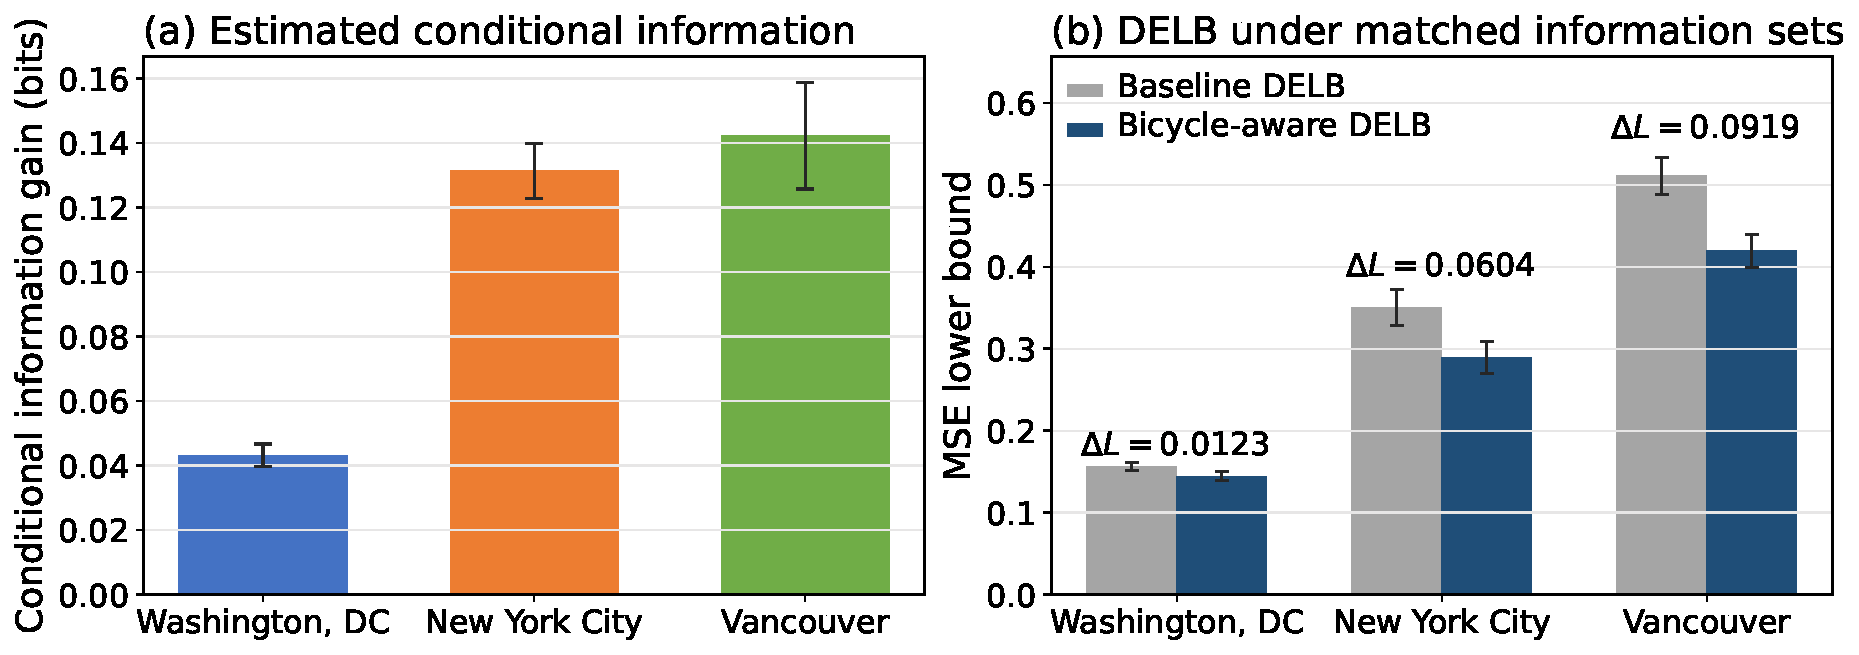
\includegraphics[width=\textwidth]{figures/e17/e17_city_cmi_delb_combined.pdf}
\caption{Primary city-level point estimates. \textbf{(a)} Miller--Madow CMI
with centered 95\% seven-day block-bootstrap intervals.
\textbf{(b)} DELB-implied MSE floors under the baseline and bicycle-aware
information sets. These intervals describe sampling variation under the
observed support; randomization calibration is reported in
Section~\ref{subsec:results_nulls}.}
\label{fig:city_information_bounds}
\end{figure}
\FloatBarrier

\begin{table}[!htbp]
\caption{City-level DELB point estimates for two training-period-frozen
analysis populations. The deployment population uses the complete
crime-supported domain; the bicycle-covered population uses its
bicycle-covered subset.}
\label{tab:co_primary_domains}
\begin{adjustwidth}{-\extralength}{0cm}
\centering
\begin{tabular*}{\linewidth}{@{\extracolsep{\fill}}llrrrrrr@{}}
\toprule
\textbf{City} & \textbf{Population} & \textbf{Grids} & \textbf{\(N\)} &
\textbf{CMI (bit)} & \textbf{\(L^0\)} & \textbf{\(L^B\)} &
\textbf{\(\Delta L\)}\\
\midrule
Washington, DC & Deployment (complete) & 186 & 203,670 & 0.0420 & 0.1535 & 0.1416 & 0.0119\\
Washington, DC & Coverage-conditioned & 181 & 198,195 & 0.0432 & 0.1567 & 0.1443 & 0.0123\\
New York City & Deployment (complete) & 806 & 882,570 & 0.0348 & 0.1382 & 0.1288 & 0.0094\\
New York City & Coverage-conditioned & 198 & 216,810 & 0.1314 & 0.3503 & 0.2898 & 0.0604\\
Vancouver & Deployment (complete) & 141 & 154,395 & 0.0377 & 0.1774 & 0.1659 & 0.0115\\
Vancouver & Coverage-conditioned & 34 & 37,230 & 0.1423 & 0.5113 & 0.4194 & 0.0919\\
\bottomrule
\end{tabular*}
\end{adjustwidth}
\end{table}


The two co-primary, training-period-frozen populations retained positive
city-level point estimates (Table~\ref{tab:co_primary_domains}). In the complete
crime-supported domain, CMI was 0.0420, 0.0348, and 0.0377 bits in
Washington, DC, New York City, and Vancouver, respectively, compared with
0.0432, 0.1314, and 0.1423 bits in the bicycle-covered domain. The
corresponding complete-domain DELB reductions were 0.0119, 0.0094, and
0.0115 MSE units, versus 0.0123, 0.0604, and 0.0919. Thus, the sign was
stable, but the magnitude in New York City and Vancouver depended strongly
on the spatial target population. This co-primary comparison concerns
city-level point estimates only; the downstream inferential experiments
retain their prespecified bicycle-covered populations.

\subsubsection{Local Estimates and Spatial Patterning}
\label{subsec:results_local_information}

Of 413 bicycle-covered cells, 339 met local eligibility criteria: 146 in
Washington, DC, 160 in New York, and 33 in Vancouver. Median local DELB
reductions were \DCLocalMedianDeltaL{}, \NYLocalMedianDeltaL{}, and
\VANLocalMedianDeltaL{} units, respectively.The sampling-uncertainty screen
was positive in 137 of 146 Washington cells, 155 of 160 New York cells,
and all 33 eligible Vancouver cells.

Spatial autocorrelation differed across cities. Global Moran's \(I\) for
the local DELB reduction was 0.164 in Washington, DC (\(p=0.002\)), 0.038 in New York City
(\(p=0.261\)), and 0.171 in Vancouver (\(p=0.022\)). Thus, local point
estimates were spatially clustered in Washington and Vancouver but not
detectably clustered in New York under the specified contiguity design.

The local table and map are reported in Supplementary Materials, Section S2.
Their colors represent
point-estimate magnitude rather than statistical significance; the
randomization analysis below evaluates whether the observed local
reductions exceed their temporal, spatial, and circular-shift references.

\subsection{Randomization Calibration and Lag Specificity}
\label{subsec:results_nulls}

The randomization analyses evaluated whether the observed CMI was unusually
large relative to three prespecified transformation-based reference
distributions. Evidence under a given design required the observed
statistic to fall in the upper tail of that reference distribution;
the reference center was not constrained to zero.

None of the nine city-by-reference comparisons rejected its corresponding
upper-tail null. Unadjusted \(p\)-value ranged from 0.903 to 1.000, and all multiplicity-adjusted
\(q\)-value were 1.000. In most comparisons, the observed CMI was below
the corresponding reference mean. At the local level, none of the 339
eligible cells passed all three randomization designs, including cells
that had passed the block-bootstrap sampling-uncertainty screen.

E17 produced the same city-level conclusion for all three entropy
estimators. Across the nine comparisons within each estimator, raw
\(p\)-values ranged from 0.980 to 1.000 for plug-in, 0.903 to 1.000 for
Miller--Madow, and 0.984 to 1.000 for Jeffreys--Dirichlet. No comparison
passed either the estimator-specific nine-test correction
(\ESeventeenWithinRejects{}/27) or the global 27-test correction
(\ESeventeenGlobalRejects{}/27). The full estimator-specific null summaries
are reported in Supplementary Materials, Section S1.

The distant-lag analysis produced similar CMI estimates. Ratios of
14-day- or 30-day-lag CMI to the matched one-day-lag CMI ranged from
\DistantRatioMin{} to \DistantRatioMax{}. Both distant-lag estimates
exceeded the one-day estimate in New York City, whereas differences
in Washington, DC and Vancouver were small and inconsistent
(Table~\ref{tab:null_calibration}). The detailed lag figure is retained in
Supplementary Materials, Section S2.

Taken together, the three randomization designs and distant-lag comparisons
did not isolate an information signal specific to recent, geographically
matched bicycle activity. The results nevertheless remain conditional on
the transformations examined; they do not constitute a general test of
conditional independence.

\begin{table}[!htbp]
\caption{Baseline-state-matched restricted randomization and semi-synthetic
calibration. Type I error and power use 50 Monte Carlo datasets and 99
randomizations per dataset under the fitted-dispersion scenario.}
\label{tab:e18_restricted_calibration}
\centering
\setlength{\tabcolsep}{2.5pt}
\begin{tabular*}{\textwidth}{@{\extracolsep{\fill}}lrrrrrrr@{}}
\toprule
\textbf{City} & \shortstack{\textbf{Observed}\\\textbf{CMI}} &
\shortstack{\textbf{Null}\\\textbf{mean}} &
\textbf{\(p\)} & \shortstack{\textbf{Type I}\\\textbf{error}} &
\shortstack{\textbf{Power at}\\\textbf{0.02 bit}} &
\shortstack{\textbf{Power at}\\\textbf{0.05 bit}} &
\shortstack{\textbf{Power at highest}\\\textbf{evaluated CMI}}\\
\midrule
Washington, DC & 0.0432 & 0.0433 & 0.599 & 0.04 & 0.10 & 0.06 &
0.48 at 0.0649 bit\\
New York City & 0.1314 & 0.1338 & 0.999 & 0.08 & 0.02 & 0.02 &
0.46 at 0.1000 bit\\
Vancouver & 0.1423 & 0.1476 & 0.994 & 0.00 & 0.02 & 0.02 &
0.30 at 0.1000 bit\\
\bottomrule
\end{tabular*}
\end{table}


The baseline-state-matched restricted randomization reached a movable-block
share of 1.00 in every city and preserved the bicycle-state marginal
exactly. Its null means were again slightly above the observed CMI
(Table~\ref{tab:e18_restricted_calibration}). The upper-tail \(p\)-values
were 0.599, 0.999, and 0.994 in Washington, DC, New York City, and
Vancouver; all three BH-adjusted \(q\)-values were 0.999. Thus, bringing
the reference closer to the baseline state did not reverse the E10
non-rejection.

The semi-synthetic results qualified that finding. Under zero population
CMI, restricted-design rejection rates ranged from 0.00 to 0.08 across
cities and dispersion settings, and every exact 95\% binomial interval
covered 0.05. However, power at 0.02 and 0.05 bit was only 0.00--0.10.
Even under the fitted-dispersion scenario, power at the highest evaluated
attainable CMI was 0.48 in Washington, DC, 0.46 in New York City, and
0.30 in Vancouver. Some requested high-CMI settings were unattainable on
the fixed empirical support and were reported at their actual maxima.
Consequently, E18 supports calibration of the restricted reference but
also shows limited detection power; its non-rejection cannot establish
conditional irrelevance.




\begin{table}[H]
\caption{\rev{Randomization-reference calibration and distant-lag diagnostics.} Randomization
\(p\)-values are upper-tail tests of whether observed CMI exceeds the
specified null distribution. Distant-lag columns report
\(\widehat I_{\mathrm{distant}}/\widehat I_{\mathrm{recent}}\).}
\label{tab:null_calibration}
\centering
\begin{tabular*}{\linewidth}{@{\extracolsep{\fill}}lrrrrr@{}}
\toprule
\textbf{City} & \multicolumn{3}{c}{\textbf{Randomization \(p\)-value}} &
\multicolumn{2}{c}{\textbf{Distant/recent CMI}}\\
\cmidrule(lr){2-4}\cmidrule(lr){5-6}
 & \textbf{Temporal} & \textbf{Spatial} & \textbf{Circular} &
\textbf{14 days} & \textbf{30 days}\\
\midrule
Washington, DC & 1.000 & 1.000 & 0.967 & 0.992 & 0.985\\
New York City & 1.000 & 0.986 & 0.993 & 1.020 & 1.052\\
Vancouver & 1.000 & 0.969 & 0.903 & 0.964 & 1.007\\
\bottomrule
\end{tabular*}
\end{table}


\begin{figure}[!t]
\begin{adjustwidth}{-\extralength}{0cm}
\centering
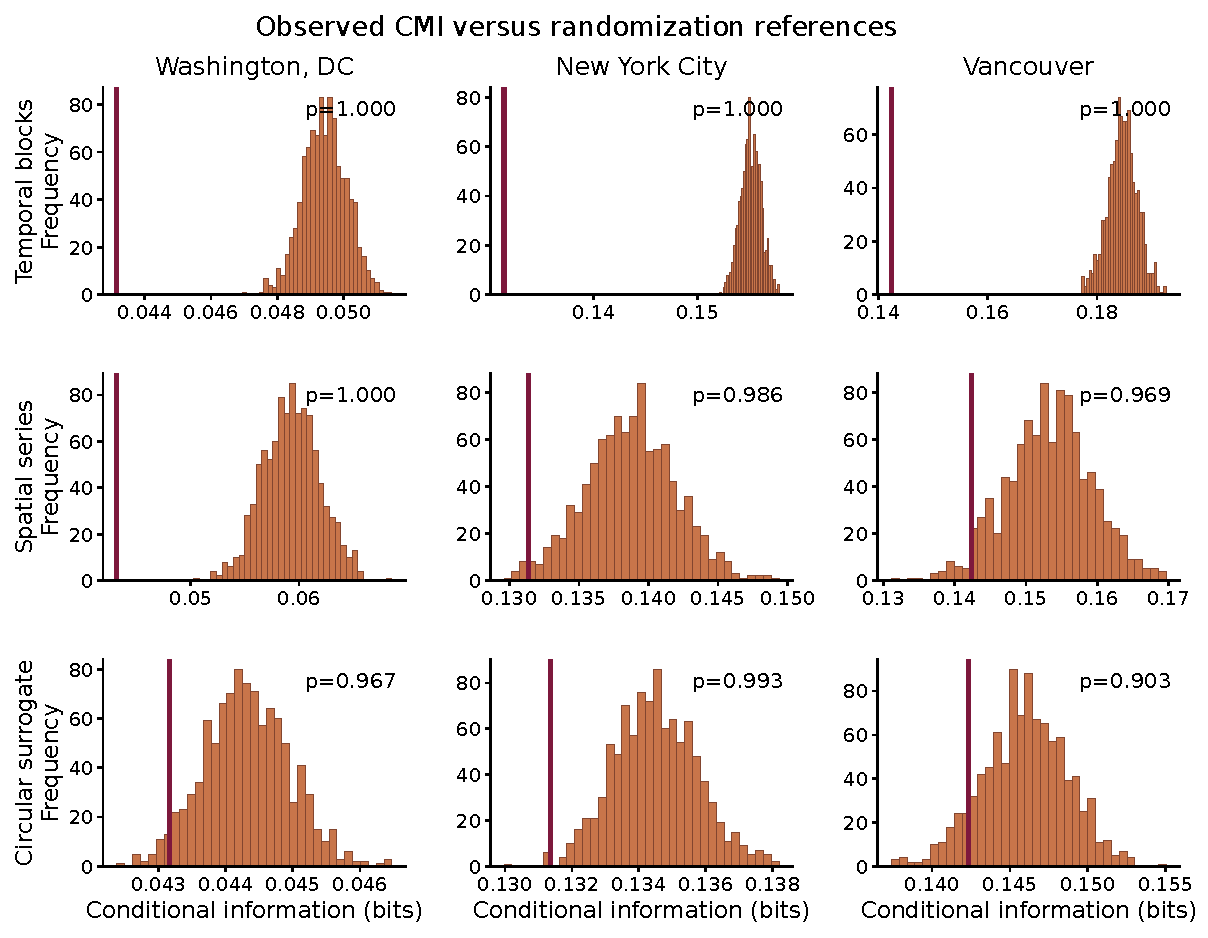
\includegraphics[width=\linewidth]{figures/e11/e10_city_null_distributions.pdf}
\end{adjustwidth}
\caption{Observed city-level CMI relative to temporal-block,
spatial-series, and circular-shift reference distributions. The observed
statistic did not exceed any prespecified upper-tail reference.}
\label{fig:city_nulls}
\end{figure}



\subsection{Spatiotemporal Scale and Sample-Size Calibration}
\label{subsec:e16_scale_results}

The multiscale analysis separated three sources of variation. Spatial
and temporal aggregation changed the prediction target, sample thinning
evaluated estimator stability within a fixed design, and randomization
compared each observed statistic with its transformation-specific reference.

Across the 18 full-sample city--space--time combinations, estimated
Miller--Madow CMI ranged from \ScaleFullCMIMin{} to \ScaleFullCMIMax{} bits,
and singleton-observation share ranged from \ScaleSingletonMin{} to \ScaleSingletonMax{}.
Every full-sample combination produced a positive estimated DELB reduction.
After deterministic area--time scaling, reductions in the implied RMSE floor
ranged from \ScaleIntensityReductionMin{} to \ScaleIntensityReductionMax{} crimes
km\(^{-2}\) day\(^{-1}\). Because aggregation changes both the outcome
distribution and the MSE unit, these values describe distinct
scale-specific targets rather than repeated estimates of one
scale-invariant quantity.

Estimator stability improved as more time blocks were retained. At the 20\%
sample fraction, the median relative deviations from the corresponding full-sample estimates
were \ScaleBoundStabilityTwenty{} for the baseline DELB, 0.646 for the
bicycle-aware DELB, 0.630 for the DELB reduction, and \ScaleCMIStabilityTwenty{} for CMI.
At the 80%
fraction, these deviations had declined to \ScaleBoundStabilityEighty{}, 0.114,
0.070 and \ScaleCMIStabilityEighty{}, respectively
(Supplementary Materials, Section S3).
These deviations measure agreement with the full-sample estimate
rather than distance from the unknown population quantity.

Randomization results were consistent across scales and sample fractions.
None of the 270 city--space--time--sample--reference tests survived either the
global or within-family FDR correction. The minimum unadjusted \(p\)-value was
\ScaleMinimumRawP{} and the minimum within-family \(q\)-value was
\ScaleMinimumWithinQ{}.
Thirty-three observed CMI values exceeded their corresponding reference
means, but none did so under temporal-block randomization.
At the prespecified full-sample scales, the New York 500 m
daily circular-shift comparison had \(p=0.006\), but its global
\(q\)-value was \(q=0.54\).

Thus, positive estimated DELB reductions occurred at every full-sample
scale, while the prespecified multiscale calibration produced no
multiplicity-adjusted evidence that the reductions were specific
to the aligned bicycle state.


\begin{table}[H]
\caption{Multiscale upper-tail randomization calibration. Discoveries use a Benjamini--Hochberg adjustment across all 270 tests.}
\label{tab:e16_randomization_summary}
\begin{adjustwidth}{-\extralength}{0cm}
\centering
\small
\begin{tabular}{lccccc}
\toprule
\textbf{Null design} & \textbf{Tests} & \textbf{Min. $p$} & \textbf{Median $p$} & \textbf{Obs. $>$ null} & \textbf{FDR discoveries}\\
\midrule
Temporal block & 90 & 0.873 & 1.000 & 0 & 0\\
Spatial series & 90 & 0.130 & 0.945 & 12 & 0\\
Circular shift & 90 & 0.005 & 0.917 & 21 & 0\\
\bottomrule
\end{tabular}
\end{adjustwidth}
\end{table}


\begin{figure}[H]
\begin{adjustwidth}{-\extralength}{0cm}
\centering
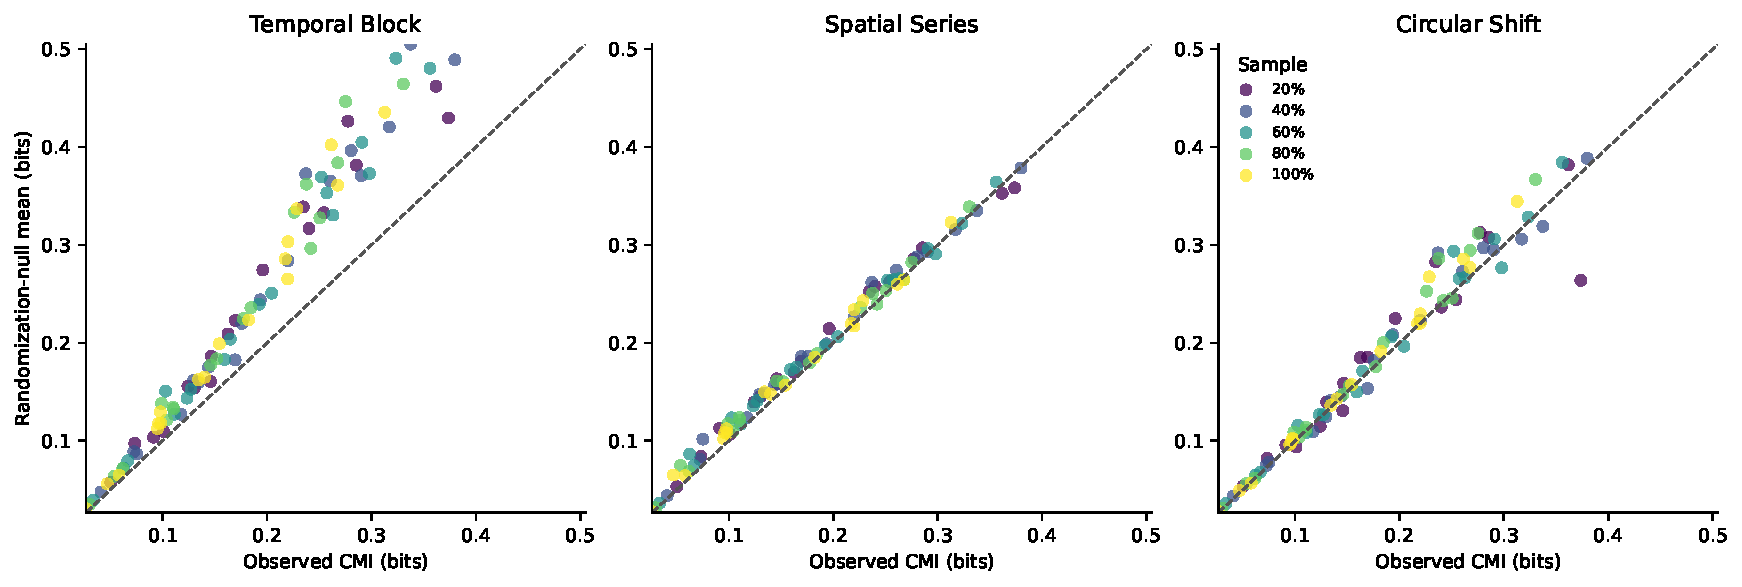
\includegraphics[width=\linewidth]{figures/e16/e16_s16_6_observed_vs_null.pdf}
\end{adjustwidth}
\caption{Observed Miller--Madow CMI versus the randomization-reference mean
across 270 city--space--time--sample--design comparisons. The dashed line is
equality; a nonzero reference center is allowed and is not population CMI.}
\label{fig:e16_observed_null}
\end{figure}


\subsection{Held-Out Prediction and Predictability Gaps}
\label{subsec:results_prediction}

Held-out prediction evaluated whether particular fitted models converted
the augmented information state into lower error on unseen observations.
The fixed July--December 2022 test set contained 75,992 grid--day observations.

Adding the bicycle state reduced the MSE point estimate in six of the 12
city--model comparisons. Three comparisons passed the adjusted
positive-improvement screen: the state-mean and Poisson gradient-boosting
models in New York City and the state-mean model in Vancouver.
The remaining model--city combinations showed either negligible change
or higher MSE after the bicycle state was added (Figure~\ref{fig:mse_improvement}).

All held-out MSE values remained above their matched DELB estimates.
The New York state-mean model narrowed the estimated Predictability Gap
by 0.001 MSE units, and New York gradient boosting narrowed it by 0.029.
All other comparisons produced negative gap changes
(Table~\ref{tab:prediction_gap_results} and Figure~\ref{fig:gap_narrowing}).

These results show that a lower estimated information-constrained
bound and lower realized error need not occur together.
The augmented state was associated with a lower estimated DELB in
every city, but only selected model--city combinations achieved lower
held-out MSE, and only two narrowed the corresponding estimated
Predictability Gap.

\begin{figure}[H]
\centering
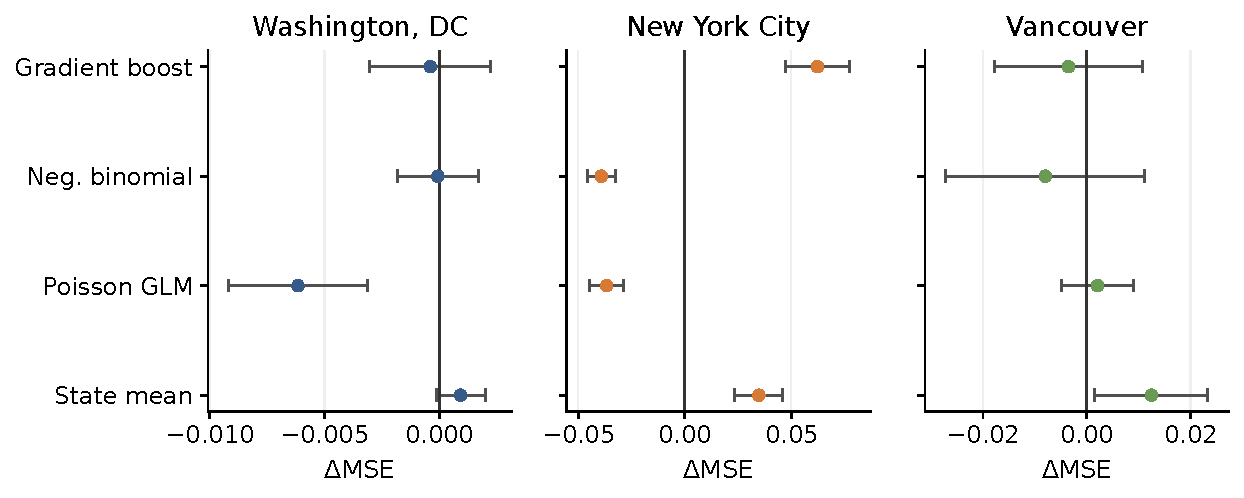
\includegraphics[width=\textwidth]{figures/e11/e06_mse_improvement.pdf}
\caption{Held-out integer-MSE change after adding lagged bicycle state.
Positive values favor the bicycle-aware specification; comparisons are
paired within city and model family.}
\label{fig:mse_improvement}
\end{figure}


\begin{table}[!htbp]
\caption{Matched held-out integer-prediction MSE, DELB, and Predictability Gap results for July--December 2022. The paired DELB column reports the baseline and bicycle-augmented lower bounds as \(L^0/L^B\). Positive \(\Delta\mathrm{MSE}\) denotes lower error after adding bicycle information. Gap narrowing is \(\Delta G=\Delta\mathrm{MSE}-\Delta L\): a positive value indicates that the model moved closer to the lower bound, whereas a negative value indicates that the estimated lower bound decreased more than the model MSE. Differences were calculated from unrounded values and then rounded for display.}
\label{tab:prediction_gap_results}
\begin{adjustwidth}{-\extralength}{0cm}
\raggedleft
\begin{tabular*}{\linewidth}{@{\extracolsep{\fill}}llrrrrrr@{}}
\toprule
\textbf{City} & \textbf{Model} & \(\boldsymbol{\mathrm{MSE}^0}\) &
\(\boldsymbol{\mathrm{MSE}^B}\) & \(\boldsymbol{L^0/L^B}\) &
\(\boldsymbol{\Delta\mathrm{MSE}}\) &
\(\boldsymbol{\Delta L}\) & \textbf{Gap narrowing}\\
\midrule
Washington, DC & State mean & \rev{0.5002} & \rev{0.4993} & 0.107/0.092 & \rev{0.0009} & 0.015 & -0.014\\
Washington, DC & Poisson GLM & \rev{0.4933} & \rev{0.4994} & 0.107/0.092 & \rev{-0.0062} & 0.015 & -0.021\\
Washington, DC & Negative-binomial GLM & \rev{0.4931} & \rev{0.4932} & 0.107/0.092 & \rev{-0.0001} & 0.015 & -0.015\\
Washington, DC & Poisson gradient boosting & \rev{0.4952} & \rev{0.4956} & 0.107/0.092 & \rev{-0.0004} & 0.015 & -0.016\\
New York City & State mean & \rev{2.0893} & \rev{2.0545} & 0.263/0.230 & \rev{0.0348} & 0.034 & 0.001\\
New York City & Poisson GLM & \rev{1.9043} & \rev{1.9410} & 0.263/0.230 & \rev{-0.0367} & 0.034 & -0.070\\
New York City & Negative-binomial GLM & \rev{1.9073} & \rev{1.9465} & 0.263/0.230 & \rev{-0.0392} & 0.034 & -0.073\\
New York City & Poisson gradient boosting & \rev{1.9010} & \rev{1.8388} & 0.263/0.230 & \rev{0.0623} & 0.034 & 0.029\\
Vancouver & State mean & \rev{1.6632} & \rev{1.6507} & 0.259/0.208 & \rev{0.0125} & 0.051 & -0.038\\
Vancouver & Poisson GLM & \rev{1.6287} & \rev{1.6266} & 0.259/0.208 & \rev{0.0021} & 0.051 & -0.049\\
Vancouver & Negative-binomial GLM & \rev{1.6138} & \rev{1.6218} & 0.259/0.208 & \rev{-0.0080} & 0.051 & -0.059\\
Vancouver & Poisson gradient boosting & \rev{1.6654} & \rev{1.6690} & 0.259/0.208 & \rev{-0.0035} & 0.051 & -0.054\\
\bottomrule
\end{tabular*}
\end{adjustwidth}
\end{table}


\begin{figure}[H]
\centering
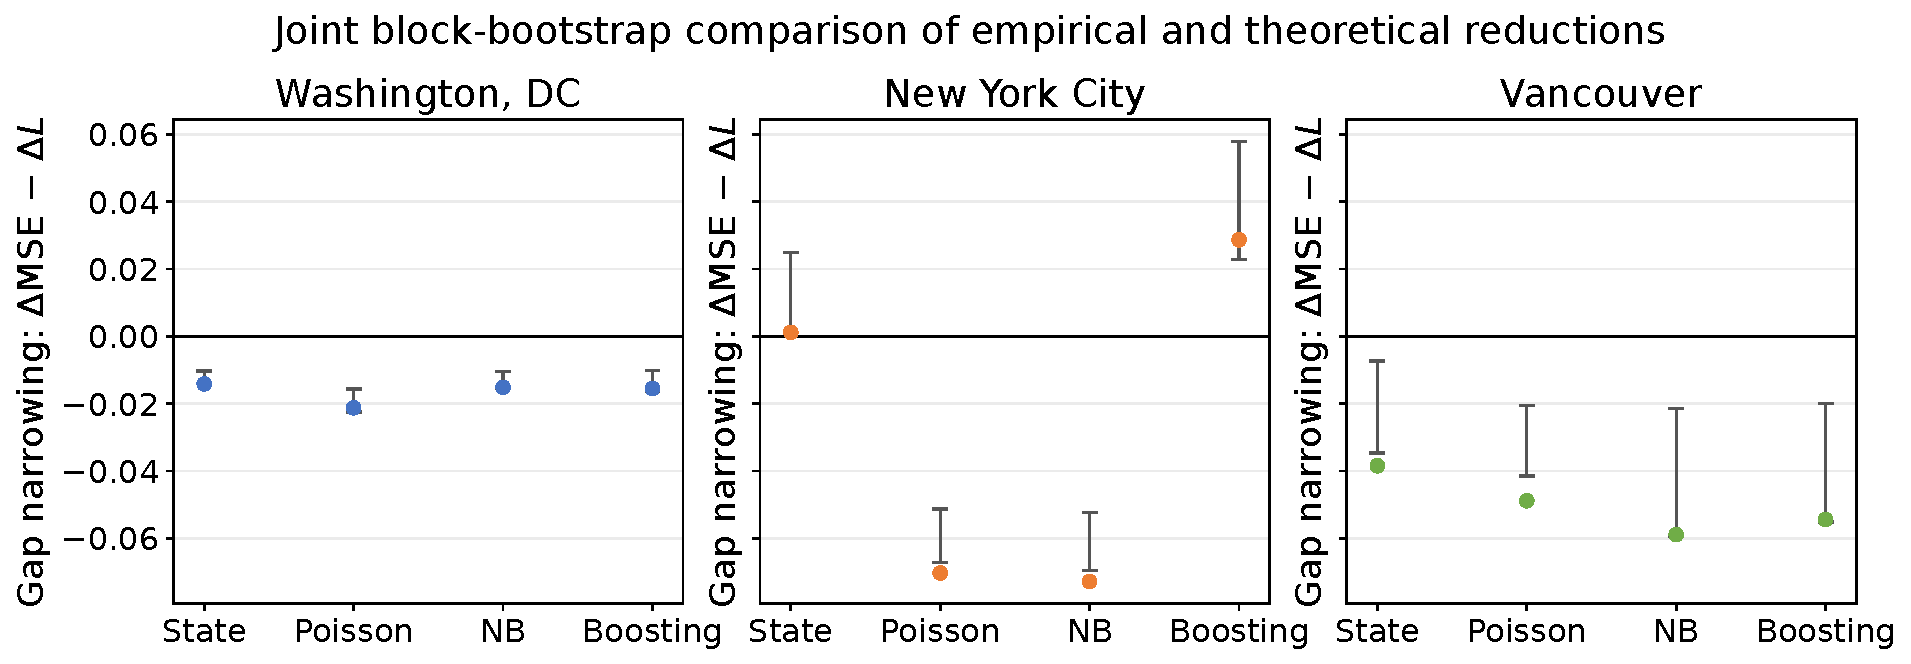
\includegraphics[width=\textwidth]{figures/e11/e07_gap_narrowing.pdf}
\caption{Predictability-gap narrowing after adding bicycle state. Positive
values mean empirical MSE fell by more than the estimated DELB; negative
values indicate a larger unused-information gap.}
\label{fig:gap_narrowing}
\end{figure}



\subsection{Secondary and Robustness Analyses}

\subsubsection{Fano Classification-Loss Comparison}
\label{subsec:results_fano}
All \FanoOracleRows{} population-oracle comparisons satisfied Fano's inequality,
and all empirical held-out modal-classifier errors remained above their
corresponding pretest Fano floors. No point-estimate violations
were observed.

Adding the bicycle state lowered the estimated Miller--Madow Fano floor
in all six city--target comparisons. Reductions ranged from \FanoFloorReductionMin{} to \FanoFloorReductionMax{}.
In contrast, held-out modal-classifier error increased in all six comparisons,
alongside increases in the number of unseen bicycle-augmented test states
(Table~\ref{tab:e14_fano_results} and Figure~\ref{fig:e14_fano}).

The opposite directions of the floor and classifier error are consistent
with the inequality. Added information can lower a population or pretest
error bound while sparse finite-sample state estimation worsens the
performance of a particular classifier. The Fano and DELB magnitudes are
not directly comparable because they concern different targets and loss
functions.




\begin{table}[!htbp]
\caption{\rev{Miller--Madow Fano floors and held-out statewise modal-classifier errors. The interval refers to the baseline-minus-bicycle floor reduction. The final column gives baseline/bicycle-aware counts of test observations assigned through the pretest global-mode fallback because their states were unseen before testing.}}
\label{tab:e14_fano_results}
\centering
\small
\setlength{\tabcolsep}{2.5pt}
\begin{tabular*}{\textwidth}{@{\extracolsep{\fill}}llccccc@{}}
\toprule
\textbf{City} & \textbf{Target} & \textbf{Base floor} & \textbf{Bike floor} & \textbf{Reduction [95\% CI]} & \textbf{Test error} & \shortstack{\textbf{Unseen test}\\\textbf{observations}}\\
\midrule
Washington, DC & Binary occurrence & 0.126 & 0.115 & 0.010 [0.010, 0.011] & 0.200/0.205 & 865/2,071\\
Washington, DC & Three-level count & 0.133 & 0.122 & 0.012 [0.011, 0.013] & 0.232/0.235 & 865/2,071\\
New York City & Binary occurrence & 0.150 & 0.124 & 0.027 [0.024, 0.029] & 0.358/0.364 & 2,058/4,408\\
New York City & Three-level count & 0.181 & 0.151 & 0.030 [0.027, 0.033] & 0.445/0.450 & 2,058/4,408\\
Vancouver & Binary occurrence & 0.200 & 0.175 & 0.025 [0.022, 0.028] & 0.326/0.335 & 234/812\\
Vancouver & Three-level count & 0.261 & 0.224 & 0.038 [0.034, 0.041] & 0.393/0.401 & 234/812\\
\bottomrule
\end{tabular*}
\end{table}


\begin{figure}[H]
\begin{adjustwidth}{-\extralength}{0cm}
\centering
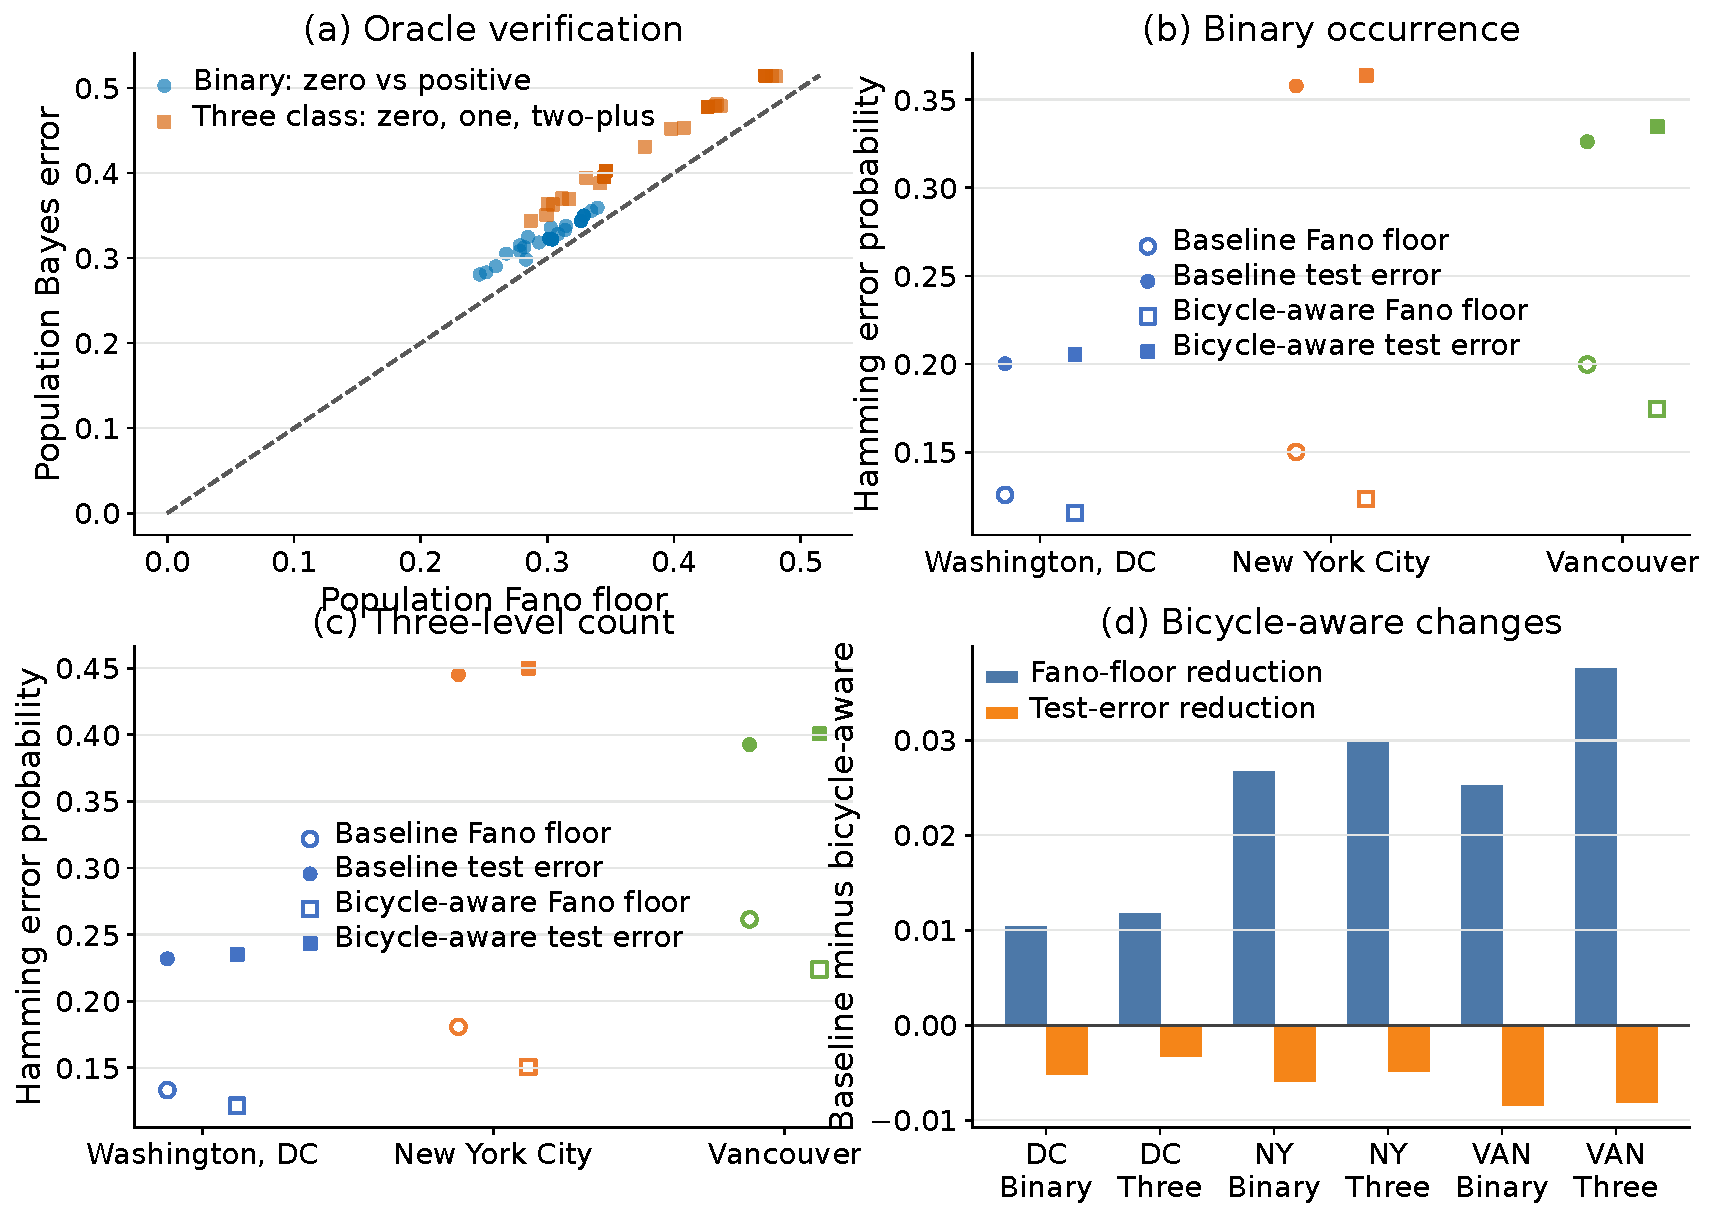
\includegraphics[width=\linewidth]{figures/s7/e14_fano_main.pdf}
\end{adjustwidth}
\caption{Fano classification-loss comparison. Oracle panels compare true
Bayes errors with true Fano floors; empirical panels compare estimated
pretest floors with held-out modal-classifier errors.}
\label{fig:e14_fano}
\end{figure}



\subsubsection{Crime-Type Heterogeneity}
\label{subsec:results_crime_types}

All \PositiveCrimeTypeTheory{} pooled city--category CMI estimates were positive.
Property theft produced the largest estimated DELB reduction in each city:
0.009 in Washington, DC, 0.045 in New York City, and 0.060 in Vancouver.
Vehicle theft and burglary produced smaller reductions
(Supplementary Materials, Section S4).

Four of the 36 matched city--crime-type--model comparisons passed the
adjusted positive-prediction screen, all in New York City. Only the
New York property-theft gradient-boosting model also narrowed the estimated
Predictability Gap. Because the primary randomization calibration was
not repeated within each crime category, these category-specific results
are treated as exploratory.



\subsubsection{Alternative Specifications and Rolling Origins}
\label{subsec:results_robustness}

The sign of the estimated DELB reduction was stable across the
prespecified theoretical alternatives. DELB reductions were positive in all
16 specifications in each city for the plug-in, Miller--Madow, and coherent
observed-support Jeffreys--Dirichlet estimators, including alternative
spatial and temporal resolutions, state mappings, estimators,
lag definitions, and bicycle-flow measures. Magnitudes across
aggregation levels are not directly comparable because the target
and MSE units change.

Rolling-origin prediction remained model- and city-dependent. New York
gradient boosting improved at all 12 monthly origins, with a mean MSE
reduction of 0.076, and the New York state-mean model improved at 11
origins, with a mean reduction of 0.030. The state-mean model improved
at eight origins in both Washington, DC and Vancouver, with mean
reductions of 0.001 and 0.006. Most GLM averages were negative. Complete
rolling-origin results are reported in Supplementary Materials, Section S5.

The alternative specifications therefore support the robustness of the
positive point-estimate pattern, while the rolling-origin results
show that conversion of the augmented state into improved prediction
depends on both city and model family.

\section{Discussion}
\label{sec:discussion}

\subsection{The DELB as an Integer-Valued Predictability Benchmark}
\label{subsec:discussion_rq1}

The first contribution of this study is an exact entropy-constrained MSE
lower bound for causal integer-valued prediction. Conditional Shannon
entropy is mapped through the inverse integer-lattice maximum-entropy
envelope, producing a model-independent benchmark for every admissible
integer-valued predictor under the specified information set and
squared-error loss.

The DELB should be interpreted carefully. It is exact in its discrete-envelope
form, but it does not
automatically equal the full Bayes risk. Universal attainment additionally
requires the prediction error to be independent of the admissible history
and to follow the moment-matched centered discrete-Gaussian distribution.
The predictor-dependent refinement accounts for residual dependence between
the error and the information set, while the two-slack decomposition
distinguishes this history-dependence component from error-distribution
shape mismatch.

More precisely, the comparison is with the infimum risk over measurable,
integer-valued, causal predictors having finite MSE under the stated
information set. The DELB does not exceed this optimal risk. If the
infimum is attained, equality holds only when an optimizing predictor
satisfies both attainment conditions. If no optimizer exists, numerical
equality of the two infima must not be described as attainment by a
predictor.

This distinction gives the DELB a diagnostic role beyond that of a scalar
benchmark. A large gap between achieved MSE and the universal DELB may
reflect remaining exploitable dependence, an unsuitable error distribution,
finite-sample model limitations, or some combination of these factors.
Consequently, the bound identifies a theoretically available region of
performance rather than guaranteeing that a practical estimator can reach
it.

The theorem is independent of the crime and bicycle application.
Numerical inversion and simulation verify the computational
implementation of the lattice envelope and its boundary cases, but the
theorem itself follows analytically. Likewise, the Fano analysis provides
a classification-loss counterpart and is not a second validation of the DELB.



\subsection{Finite-Sample Information Gain Requires Its Own Inferential Layer}
\label{subsec:discussion_rq2}

At the population level, adding side information reduces conditional
entropy by exactly its CMI with the target given the baseline information.
Monotonicity of the inverse lattice envelope then orders the corresponding
DELBs. This population statement is straightforward; estimating it from
sparse conditional states is not.

The known-truth simulations show that positive estimated CMI can
arise under zero population CMI. Adding a discretized variable divides each
baseline state into a larger number of joint states, many of which may be
weakly occupied or observed only once. Standard corrections reduce some
of this bias but do not remove the dependence of the estimate on state-space
geometry and sample size.

The estimator sensitivity analysis leads to the same caution. Plugin,
Miller--Madow, and observed-support Jeffreys--Dirichlet estimates produced
positive DELB reductions for all 16 prespecified specifications in each
city. Yet E17 found no rejection under any estimator, whether false
discovery rates were controlled within its nine city--null-design tests
or across all 27 estimator--city--design tests. The Jeffreys result is a
sensitivity check over observed support, not a reconstruction of
unobserved states.

A second distinction concerns randomization. A transformation-based
reference distribution is generated by repeatedly changing the observed
data structure and recomputing both the statistic and its support.
Its center therefore need not be zero and should not be interpreted as
either population CMI or a direct estimate of estimator bias. Valid
interpretation is specific to the estimator, transformation, sample,
and support produced by the randomization design.

The empirical support diagnostics reinforce this point. Effective
conditional degrees of freedom were strongly associated with the
reference-distribution center, and changes in support under randomization
were associated with differences between observed and reference CMI. These
findings do not provide a universal analytic bias formula, but they show
why comparing an estimated CMI directly with zero can be misleading
in sparse nested panels.


The resulting evidence hierarchy is therefore:
\begin{equation}
\begin{gathered}
\text{population DELB/CMI}
\longrightarrow
\text{finite-sample estimate}
\longrightarrow
\text{estimator behavior}\\
\longrightarrow
\text{design-conditioned reference}
\longrightarrow
\text{realized prediction error}.
\end{gathered}
\label{eq:discussion_inference_chain}
\end{equation}
Each stage answers a different question. A positive estimate describes
the observed partition; a randomization comparison evaluates a specified
null mechanism; and held-out prediction evaluates a particular fitted model.
None can substitute automatically for the others.


\subsection{What the Bicycle--Crime Analysis Does and Does Not Establish}
\label{subsec:discussion_rq3}

The urban results contain a strong descriptive pattern. Adding lagged
bicycle state reduced estimated conditional entropy and the corresponding
DELB in every city, every full-sample spatial--temporal scale, all 16
alternative theoretical specifications, and all exploratory crime categories.
The local estimates also showed spatial clustering in Washington, DC and
Vancouver. These results indicate that bicycle-augmented state partitions
consistently separate crime-count distributions more finely in the observed
samples.

The training-period-frozen analysis-domain comparison preserved the
direction of this pattern but changed its magnitude. Expanding from the
training-period bicycle-covered domain to the complete training-period
crime domain attenuated CMI and DELB reductions most strongly in New York
and Vancouver. The estimate therefore depends on the spatial target
population fixed before validation and testing; this domain contrast has
no causal interpretation.

The calibrated evidence was substantially weaker. None of the city-level
or local comparisons distinguished the observed CMI from all prespecified
temporal, spatial, and circular-shift references. Distant bicycle lags
yielded estimates comparable with the one-day lag, and none of the 270
multiscale randomization tests survived FDR correction. Thus, the present
design does not isolate an information contribution specific to recent,
geographically aligned bicycle mobility.

This finding should not be interpreted as proof that bicycle activity is
conditionally irrelevant to crime. The transformations are diagnostic
rather than exact conditional randomization procedures that preserve the
complete mobility distribution within every baseline state. Bicycle
use contains slow seasonal patterns, system-wide operational changes,
weather responses, pandemic-period shifts, and other common temporal
structure. These components can remain present in both recent and
transformed mobility series.

The baseline-state-matched restricted randomization reached the same
non-rejection while preserving grid and calendar strata more closely.
Its semi-synthetic Type I error was compatible with the nominal level, but
power remained low at CMI magnitudes comparable with the smaller empirical
signals. The added experiment therefore strengthens the calibration audit,
not a claim that mobility is conditionally irrelevant.

A more precise interpretation is therefore that the positive estimated
DELB reductions cannot, under the current calibration, be uniquely
attributed to recent bicycle-specific activity. This is a limit on
empirical attribution rather than a rejection of mobility information
in general.



\subsection{Theoretical Opportunity and Realized Prediction Are Different}
\label{subsec:discussion_prediction}

The held-out analyses illustrate why a population lower bound and a
fitted model's error must be evaluated separately. Adding information
can lower the best entropy-constrained error benchmark even when a
particular estimator cannot exploit that information from a finite sample.
Conversely, a model may improve by using seasonal or proxy structure
without establishing a bicycle-specific population CMI.

This distinction appeared clearly in the results. Bicycle-augmented DELBs
declined in all cities, whereas held-out improvements varied across models
and locations. Only two New York models reduced realized MSE by more than
the estimated DELB reduction and therefore narrowed the Predictability Gap.
The Fano comparison showed the same phenomenon under classification loss:
every estimated augmented floor declined, while the statewise modal
classifier worsened in all comparisons as unseen augmented states became
more frequent.

The Predictability Gap is consequently useful as a matched accounting
quantity rather than as an independent universal metric. Both MSE and
DELB must use the same target, forecast horizon, information set,
evaluation sample, and loss. A negative change in the gap does not
violate the lower bound; it indicates that the fitted model did not
realize the additional theoretical opportunity implied by the estimated
information state.

\subsection{Practical Implications for Urban Data and Forecasting Systems}
\label{subsec:practical_implications}

For urban analytics teams, the results support a staged data-value
assessment rather than a binary decision based on one fitted model.
Table~\ref{tab:practical_decision_framework} translates the evidence layers
into four operational questions. DELB first measures whether a candidate
source changes the estimated model-independent opportunity set. Support
diagnostics and randomization then assess whether that change is
distinguishable under explicit finite-sample references. Matched held-out
models finally determine whether an available forecasting system can use
the source in the deployment population.

\begin{table}[!htbp]
\caption{Practical decision framework for evaluating an added urban data
source in an integer-count forecasting system.}
\label{tab:practical_decision_framework}
\centering
\setlength{\tabcolsep}{3.5pt}
\begin{tabularx}{\textwidth}{
>{\RaggedRight\arraybackslash}p{2.75cm}
>{\RaggedRight\arraybackslash}X
>{\RaggedRight\arraybackslash}X
>{\RaggedRight\arraybackslash}p{3.15cm}}
\toprule
\textbf{Decision question} & \textbf{Required evidence} &
\textbf{Operational response} & \textbf{Boundary}\\
\midrule
Does the source create an estimated prediction opportunity? &
DELB and CMI point estimates in frozen target populations &
Retain the source for calibrated evaluation if the estimated floor
declines materially & Point estimates alone are insufficient for
source attribution or realized benefit\\
Is the apparent gain distinguishable from finite-sample structure? &
Support diagnostics, known-truth calibration, and design-matched
randomization & Attribute the gain only to the tested design and only when
calibration and power support separation & Low-powered non-rejection is
inconclusive; randomization provides no causal identification\\
Can available models use the source on unseen data? &
Matched held-out models with identical targets, samples, tuning rules, and
loss & Deploy only city--model combinations showing stable held-out benefit;
monitor the Predictability Gap & Model-specific gains require separate
validation across cities and model families\\
Does value persist outside the service footprint? &
Training-period-frozen coverage-conditioned and complete crime-supported
deployment populations &
Report both populations and treat coverage as part of the data product &
Service-area estimates apply only to covered locations\\
\bottomrule
\end{tabularx}
\end{table}


This sequence matters for procurement and engineering. A positive DELB
reduction can justify retaining a data source for further evaluation, but
not paying for, integrating, or operationalizing it on that basis alone.
In the present application, the large bicycle-domain reductions in New
York City and Vancouver attenuated in the complete crime-supported
populations, and the calibrated tests did not isolate a bicycle-specific
signal. Coverage, state support, and calibration should therefore be
treated as properties of the data product, not as post hoc sensitivity
checks.

Deployment decisions should also remain model and city specific. The
New York state-mean and gradient-boosting models narrowed the
Predictability Gap, whereas the remaining city--model combinations did
not. A practical pipeline should consequently preserve a baseline model,
evaluate the added source on a frozen holdout period, monitor both
\(\Delta\operatorname{MSE}\) and \(\Delta G\), and withdraw the added
feature when its benefit does not persist under rolling evaluation.
The DELB is useful here as an opportunity budget: it identifies how much
the estimated floor moved, while the gap shows whether the fitted system
converted that movement into realized accuracy.

These implications concern forecasting-system evaluation, not operational
policing decisions. The analysis is aggregate, noncausal, and based on a
mode-specific mobility proxy. It does not identify individuals, locations
that should receive enforcement, or the effect of bicycle activity on
crime. Any public-sector use would require separate fairness, privacy,
governance, and causal-impact assessment beyond the scope of the DELB
workflow.



\subsection{Methodological Contribution and Scope}
\label{subsec:discussion_contributions}

The theoretical contribution is not a new discovery of the discrete-Gaussian
extremizer, the lattice correction, the information-projection identity,
or Fano's inequality. It is the integration of established ingredients into
a four-part framework for causal integer-valued prediction:

\begin{enumerate}
\item an exact inverse-lattice MSE lower bound;
\item a predictor-dependent refinement;
\item necessary and sufficient attainment conditions; and
\item a two-component decomposition of nonattainment.
\end{enumerate}
The empirical contribution is the connection of this population theory
to a reproducible finite-sample evidence strategy. This connection is
important because entropy-based prediction limits are often estimated
precisely in settings where the state space is large relative to the
available sample. Without support diagnostics and design-matched calibration,
apparent reductions in a theoretical floor may be overstated as verified
information gain.

The DELB is narrower than general Bayes-risk or rate--distortion theory.
It assumes integer-valued targets, squared-error loss, and a discrete
representation of the conditioning state. This narrower scope permits
an explicit lattice envelope and interpretable equality conditions,
but it also makes entropy estimation vulnerable to sparse support.
The same trade-off is likely to arise in demand forecasting,
epidemiological counts, traffic incidents, service arrivals,
and other integer-valued systems.



\subsection{Limitations and Future Directions}
\label{subsec:limitations}

Several limitations concern the empirical data. Shared-bicycle trips are a
mode-specific trace of public-space activity rather than a census of
ambient population. Coverage depends on service boundaries, station
locations, adoption, system rebalancing, weather, endpoint completeness,
and recording practices. Crime data are also affected by victim reporting,
police classification, and jurisdiction-specific definitions. The 2020--2022
period includes pandemic-related structural change, and associations at
the 1 km grid--day level do not support individual-level inference.

Other limitations arise from the inferential design. The randomization
procedures do not preserve the exact conditional distribution of mobility
within every baseline state and therefore should be interpreted as
transformation-specific diagnostics rather than exact
conditional-independence tests. The known-truth simulation
spans a finite factorial family, and the support regressions
are descriptive diagnostics rather than analytic bias corrections.
The E18 semi-synthetic study used six representative grids, 365 days,
50 Monte Carlo datasets per cell, and 99 randomizations per dataset.
Its binomial intervals are correspondingly wide, several requested CMI
levels were not attainable on the fixed empirical support, and its low
power prevents interpreting empirical non-rejection as evidence of no
conditional information.
The pretest Fano distribution may differ from the test-period population.
For the multiscale randomization analysis below the full sample,
computation was restricted to one prespecified thinning path, although
estimator stability was examined over 50 paths.

Spatial and temporal aggregation also changes the target distribution.
Area--time normalization changes units but does not transform daily, weekly,
500 m, and 2 km outcomes into repeated measurements of one scale-free
population quantity. Claims of a universal scale law would require a
separate theoretical definition and study design.

Future work could reduce state sparsity through shrinkage, hierarchical
pooling, Bayesian or frequentist partial pooling, and cross-fitting.
More conditional surrogate designs could preserve mobility distributions
within baseline states more closely. Empirical extensions should
incorporate additional mobility modes, pedestrian activity, transit use,
weather, and post-2022 observations while preserving matched causal
information sets. Theoretical extensions include sharper multivariate
lattice envelopes, alternative integer-valued loss functions, and bounds
for dependent vector count processes.





\section{Conclusions}
\label{sec:conclusions}

This study formulated the Discrete Entropy Lower Bound for causal
integer-valued prediction. By inverting the exact integer-lattice
maximum-entropy envelope, the DELB maps conditional Shannon entropy
to a model-independent, entropy-constrained MSE lower bound.
The framework further provides a predictor-dependent refinement,
necessary and sufficient attainment conditions, and a two-component
decomposition that separates residual history dependence from
error-distribution shape mismatch.

The study also established a finite-sample evidence strategy for
evaluating changes in this bound after side information is added.
Population CMI, estimated CMI, estimator bias, transformation-specific
randomization references, and achieved prediction error are distinct
quantities. Known-truth simulations and support diagnostics showed that
sparse nested states can produce positive CMI estimates and nonzero
randomization centers even under a population null, making design-matched
calibration essential.

In the three urban panels, lagged bicycle information consistently
lowered estimated DELBs across cities, spatial and temporal scales,
crime categories, and alternative specifications. However,
the observed reductions were not distinguishable from the prespecified
temporal, spatial, or circular-shift references after calibration, and
they did not translate uniformly into lower held-out prediction error.
The findings therefore do not establish a recent bicycle-specific
reduction in the population prediction bound, nor do they imply that
bicycle mobility is predictively irrelevant. Instead, they illustrate
the central methodological distinction of this study: a lower estimated
uncertainty bound, calibrated evidence of added information, and improved
realized prediction are separate claims requiring separate evidence.
More broadly, the DELB provides a rigorous framework for studying
information-theoretic prediction floors and finite-sample information
value in crime counts and other integer-valued stochastic systems. In
practice, it supports a staged decision process in which estimated
opportunity, calibrated separation, and realized held-out benefit must be
established separately before an added urban data source is deployed.


% The original planning scaffold is retained below for provenance but is
% excluded from compilation after E11 replaced it with evidence-backed text.

\supplementary{The independent Supplementary Materials file contains
estimator sensitivity and the training-period-frozen decision-population comparison,
local and lag-specificity details, sample-size and multiscale analyses,
crime-type heterogeneity, rolling-origin results, and additional
descriptive and finite-sample figures.}

\authorcontributions{\rev{Concept and design: M.D., Y.Z.;
    data collection: M.D.; analysis and interpretation of results: M.D.;
    original manuscript draft: M.D.; manuscript review and editing: Y.L., B.G.;
    supervision and internal resource support: Z.Y.}
    All authors have read and agreed to the published version of the
    manuscript.}

\funding{\rev{This research received no external funding. Z.Y. provided internal or personal resources for the work; no external grant number applies.}}

\institutionalreview{Not applicable.}

\informedconsent{Not applicable.}

\dataavailability{The source data are available from the District of
Columbia, New York City, and Vancouver police open-data portals and from the
Capital Bikeshare, Citi Bike, and Mobi system-data portals cited in
Section~\ref{subsec:data_sources} (all accessed 18 July 2026). The
reproducible analysis project preserves source-file hashes, standardized
schemas, reason-coded exclusions, configurations, and scripts. \rev{A versioned
archive of analysis code, configurations, tests, and 24 anonymized joint-state
frequency tables is publicly available at
\url{https://doi.org/10.5281/zenodo.22936346}. The deposited tables permit
independent recalculation of the primary city--domain--period entropy, CMI,
and DELB point
estimates. The archive is not a complete city-data reproduction package: it
does not contain the inputs needed to rerun bootstrap intervals,
randomization tests, multiscale or local analyses, or held-out model fitting.
The public GitHub repository at
\url{https://github.com/eveyear/delb-urban-crime-prediction} provides the
revised manuscript source and analysis code, with the same data-reuse
limitations as the archive.} Raw and
processed data are not redistributed; users must obtain them from the cited
providers and comply with the providers' conditions.}

\acknowledgments{The authors thank the public agencies and bicycle-system
operators that made the underlying data available.}

\conflictsofinterest{The authors declare no conflicts of interest.}

\abbreviations{Abbreviations}{%
The following abbreviations are used in this manuscript:\\
\noindent
\begin{tabular}{@{}ll}
CMI & Conditional mutual information\\
DELB & Discrete Entropy Lower Bound\\
FDR & False discovery rate\\
GLM & Generalized linear model\\
KL & Kullback--Leibler\\
MAE & Mean absolute error\\
MSE & Mean squared error\\
RMSE & Root mean squared error
\end{tabular}
}

% Superseded planning appendix retained only as an uncompiled source record.

\begin{adjustwidth}{-\extralength}{0cm}
\reftitle{References}

% References follow the MDPI ACS-style author--year--volume--pages format.
\begin{thebibliography}{999}
\fontsize{8.0}{8.6}\selectfont

\bibitem{kounadi2020review}
Kounadi, O.; Ristea, A.; Araujo, A., Jr.; Leitner, M. A systematic review
on spatial crime forecasting. \emph{Crime Sci.} \textbf{2020}, \emph{9}, 7.
\url{https://doi.org/10.1186/s40163-020-00116-7}.

\bibitem{du2023review}
Du, Y.; Ding, N. A systematic review of multi-scale spatio-temporal crime prediction methods. \emph{ISPRS Int. J. Geo-Inf.} \textbf{2023}, \emph{12}, 209. \url{https://doi.org/10.3390/ijgi12060209}.

\bibitem{mandalapu2023review}
Mandalapu, V.; Elluri, L.; Vyas, P.; Roy, N. Crime prediction using machine learning and deep learning: A systematic review and future directions. \emph{IEEE Access} \textbf{2023}, \emph{11}, 60153--60170. \url{https://doi.org/10.1109/ACCESS.2023.3286344}.

\bibitem{alves2018crime}
Alves, L.G.A.; Ribeiro, H.V.; Rodrigues, F.A. Crime prediction through
urban metrics and statistical learning. \emph{Phys. A} \textbf{2018},
\emph{505}, 435--443.
\url{https://doi.org/10.1016/j.physa.2018.03.084}.

\bibitem{angbera2023model}
Angbera, A.; Chan, H.Y. Model for spatiotemporal crime prediction with
improved deep learning. \emph{Comput. Inform.} \textbf{2023}, \emph{42},
568--590. \url{https://doi.org/10.31577/cai_2023_3_568}.

\bibitem{huang2018deepcrime}
Huang, C.; Zhang, J.; Zheng, Y.; Chawla, N.V. DeepCrime: Attentive
hierarchical recurrent networks for crime prediction. In
\emph{Proceedings of the 27th ACM International Conference on Information
and Knowledge Management}, Torino, Italy, 22--26 October 2018;
pp. 1423--1432. \url{https://doi.org/10.1145/3269206.3271793}.

\bibitem{deng2023risk}
Deng, Y.; He, R.-X.; Liu, Y. Crime risk prediction incorporating geographical spatiotemporal dependency into machine learning models. \emph{Inf. Sci.} \textbf{2023}, \emph{646}, 119414. \url{https://doi.org/10.1016/j.ins.2023.119414}.

\bibitem{jing2024multiscale}
Jing, C.; Lv, X.; Wang, Y.; Qin, M.; Jin, S.; Wu, S.; Xu, G. A deep multi-scale neural networks for crime hotspot mapping prediction. \emph{Comput. Environ. Urban Syst.} \textbf{2024}, \emph{109}, 102089. \url{https://doi.org/10.1016/j.compenvurbsys.2024.102089}.

\bibitem{wang2025mragnn}
Wang, S.; Zhang, Y.; Piao, X.; Lin, X.; Hu, Y.; Yin, B. MRAGNN: Refining urban spatio-temporal prediction of crime occurrence with multi-type crime correlation learning. \emph{Expert Syst. Appl.} \textbf{2025}, \emph{265}, 125940. \url{https://doi.org/10.1016/j.eswa.2024.125940}.

\bibitem{butt2025start}
Butt, U.M.; Letchmunan, S.; Ali, M.; Sherazi, H.H.R. START: A
spatiotemporal autoregressive transformer for enhancing crime prediction
accuracy. \emph{IEEE Trans. Comput. Soc. Syst.} \textbf{2025}, \emph{12},
4650--4664. \url{https://doi.org/10.1109/TCSS.2025.3550196}.

\bibitem{cui2026transfer}
Cui, C.; Zheng, Z.; Du, H.; Wang, W. Dynamic transfer learning with co-occurrence-guided multi-source fusion for urban spatio-temporal crime prediction. \emph{Front. Big Data} \textbf{2026}, \emph{9}, 1697392. \url{https://doi.org/10.3389/fdata.2026.1697392}.

\bibitem{hu2023fusion}
Hu, K.; Li, L.; Tao, X.; Vel\'asquez, J.D.; Delaney, P. Information fusion in crime event analysis: A decade survey on data, features and models. \emph{Inf. Fusion} \textbf{2023}, \emph{100}, 101904. \url{https://doi.org/10.1016/j.inffus.2023.101904}.

\bibitem{cesario2024multidensity}
Cesario, E.; Lindia, P.; Vinci, A. Multi-density crime predictor: An approach to forecast criminal activities in multi-density crime hotspots. \emph{J. Big Data} \textbf{2024}, \emph{11}, 1--39. \url{https://doi.org/10.1186/s40537-024-00935-4}.

\bibitem{amarante2025steval}
Amarante, G.; Pimenta, M.; Andrade, Y.; Senna, M.; Menezes, R.; Faria, A.H.; Vilas-Boas, M.; Martins, F.; et al. STEval: A framework for evaluating spatio-temporal crime prediction models. \emph{Eng. Appl. Artif. Intell.} \textbf{2025}, \emph{162}, 112123. \url{https://doi.org/10.1016/j.engappai.2025.112123}.

\bibitem{huo2025traffic}
Huo, J.; Chen, L.; Wang, L. A context knowledge guided transformer framework
for long-term traffic prediction. \emph{CCF Trans. Pervasive Comput.
Interact.} \textbf{2025}, \emph{7}, 263--273.
\url{https://doi.org/10.1007/s42486-025-00192-1}.

\bibitem{zhao2025bike}
Zhao, Y.; Du, B.; Luo, M.; Wen, H. Robust spatio-temporal demand prediction
for bike-sharing systems with dynamic hierarchical structure.
\emph{CCF Trans. Pervasive Comput. Interact.} \textbf{2025}, \emph{7},
229--245. \url{https://doi.org/10.1007/s42486-024-00167-8}.

\bibitem{fang2025uctb}
Fang, J.; Chen, L.; Chai, D.; Hong, Y.; Xie, X.; Chen, L.; Wang, L.
UCTB: An urban computing tool box for all-in-one spatiotemporal prediction
solution. \emph{CCF Trans. Pervasive Comput. Interact.} \textbf{2025},
\emph{7}, 392--412.
\url{https://doi.org/10.1007/s42486-025-00187-y}.

\bibitem{shannon1948}
Shannon, C.E. A mathematical theory of communication. \emph{Bell Syst. Tech. J.} \textbf{1948}, \emph{27}, 379--423, 623--656.

\bibitem{cover_thomas}
Cover, T.M.; Thomas, J.A. \emph{Elements of Information Theory}, 2nd ed.;
Wiley-Interscience: Hoboken, NJ, USA, 2006.
\url{https://doi.org/10.1002/047174882X}.

\bibitem{song2010limits}
Song, C.; Qu, Z.; Blumm, N.; Barab\'asi, A.-L. Limits of predictability
in human mobility. \emph{Science} \textbf{2010}, \emph{327}, 1018--1021.
\url{https://doi.org/10.1126/science.1177170}.

\bibitem{li2022traffic}
Li, G.; Knoop, V.L.; van Lint, H. Estimate the limit of predictability in
short-term traffic forecasting: An entropy-based approach.
\emph{Transp. Res. Part C Emerg. Technol.} \textbf{2022}, \emph{138},
103607. \url{https://doi.org/10.1016/j.trc.2022.103607}.

\bibitem{fang_variance_bounds}
Fang, S.; Skoglund, M.; Johansson, K.H.; Ishii, H.; Zhu, Q.
Generic variance bounds on estimation and prediction errors in time series
analysis: An entropy perspective. In \emph{Proceedings of the 2019 IEEE
Information Theory Workshop (ITW)}, Visby, Sweden, 25--28 August 2019;
pp. 1--5. \url{https://doi.org/10.1109/ITW44776.2019.8989240}.

\bibitem{ayers2025complexity}
Ayers, J.; Hahnloser, R.; Ulrich, J.; Krapp, L.S.; Nitschke, R.; Stoll, S.;
Bickel, B.; Furrer, R. Time-series random process complexity ranking using a
bound on conditional differential entropy. \emph{arXiv} \textbf{2025},
arXiv:2510.20551. \url{https://doi.org/10.48550/arXiv.2510.20551}.

\bibitem{hauser2026dmd}
Hauser, T.; H\"olz, J. Entropy based lower dimension bounds for finite-time
prediction of Dynamic Mode Decomposition algorithms. \emph{arXiv}
\textbf{2025}, arXiv:2504.20269, revised 22 March 2026.
\url{https://doi.org/10.48550/arXiv.2504.20269}.

\bibitem{massey_integer_entropy}
Massey, J.L. On the entropy of integer-valued random variables. In
\emph{Proceedings of the 1988 Beijing International Workshop on Information
Theory}, Beijing, China, 4--7 July 1988; pp. C1.1--C1.4.

\bibitem{rioul_massey}
Rioul, O. Variations on a theme by Massey.
\emph{IEEE Trans. Inf. Theory} \textbf{2022}, \emph{68}, 2813--2828.
\url{https://doi.org/10.1109/TIT.2022.3141264}.

\bibitem{shannon_rate_distortion}
Shannon, C.E. Coding theorems for a discrete source with a fidelity
criterion. \emph{IRE Natl. Conv. Rec.} \textbf{1959}, \emph{7},
142--163.

\bibitem{chen_bayes_risk}
Chen, X.; Guntuboyina, A.; Zhang, Y. On Bayes risk lower bounds.
\emph{J. Mach. Learn. Res.} \textbf{2016}, \emph{17}, 1--58.
\url{https://www.jmlr.org/papers/v17/16-185.html}.

\bibitem{jeong_ziv_zakai}
Jeong, M.; Dytso, A.; Cardone, M. A comprehensive study on Ziv--Zakai
lower bounds on the MMSE. \emph{IEEE Trans. Inf. Theory} \textbf{2025},
\emph{71}, 3214--3236.
\url{https://doi.org/10.1109/TIT.2025.3541987}.

\bibitem{paninski2003}
Paninski, L. Estimation of entropy and mutual information. \emph{Neural Comput.} \textbf{2003}, \emph{15}, 1191--1253. \url{https://doi.org/10.1162/089976603321780272}.

\bibitem{calcagnile2026benchmark}
Calcagnile, L.M.; Di Garbo, A.; Galatolo, S. A benchmark for entropy
estimators. \emph{Entropy} \textbf{2026}, \emph{28}, 311.
\url{https://doi.org/10.3390/e28030311}.

\bibitem{zan2022cmi}
Zan, L.; Meynaoui, A.; Assaad, C.K.; Devijver, E.; Gaussier, E. A conditional mutual information estimator for mixed data and an associated conditional independence test. \emph{Entropy} \textbf{2022}, \emph{24}, 1234. \url{https://doi.org/10.3390/e24091234}.

\bibitem{runge2018cmi}
Runge, J. Conditional independence testing based on a nearest-neighbor estimator of conditional mutual information. \emph{Proc. Mach. Learn. Res.} \textbf{2018}, \emph{84}, 938--947. \url{https://proceedings.mlr.press/v84/runge18a.html}.

\bibitem{li2023nncit}
Li, S.; Chen, Z.; Zhu, H.; Wang, C.D.; Wen, W. Nearest-neighbor sampling based conditional independence testing. \emph{Proc. AAAI Conf. Artif. Intell.} \textbf{2023}, \emph{37}, 8631--8639. \url{https://doi.org/10.1609/aaai.v37i7.26039}.

\bibitem{ernst2004permutation}
Ernst, M.D. Permutation methods: A basis for exact inference. \emph{Stat. Sci.} \textbf{2004}, \emph{19}, 676--685. \url{https://doi.org/10.1214/088342304000000396}.

\bibitem{cohen1979routine}
Cohen, L.E.; Felson, M. Social change and crime rate trends: A routine
activity approach. \emph{Am. Sociol. Rev.} \textbf{1979}, \emph{44},
588--608. \url{https://doi.org/10.2307/2094589}.

\bibitem{malleson2016ambient}
Malleson, N.; Andresen, M.A. Exploring the impact of ambient population
measures on London crime hotspots. \emph{J. Crim. Justice} \textbf{2016},
\emph{46}, 52--63.
\url{https://doi.org/10.1016/j.jcrimjus.2016.03.002}.

\bibitem{song2019legal}
Song, G.; Bernasco, W.; Liu, L.; Xiao, L.; Zhou, S.; Liao, W. Crime feeds
on legal activities: Daily mobility flows help to explain thieves' target
location choices. \emph{J. Quant. Criminol.} \textbf{2019}, \emph{35},
831--854. \url{https://doi.org/10.1007/s10940-019-09406-z}.

\bibitem{kadar2018mining}
Kadar, C.; Pletikosa, I. Mining large-scale human mobility data for long-term
crime prediction. \emph{EPJ Data Sci.} \textbf{2018}, \emph{7}, 26.
\url{https://doi.org/10.1140/epjds/s13688-018-0150-z}.

\bibitem{kadar2020mobility}
Kadar, C.; Feuerriegel, S.; Noulas, A.; Mascolo, C. Leveraging mobility
flows from location technology platforms to test crime pattern theory in
large cities. \emph{Proc. Int. AAAI Conf. Web Soc. Media} \textbf{2020},
\emph{14}, 339--350.
\url{https://doi.org/10.1609/icwsm.v14i1.7304}.

\bibitem{wu2022mobility}
Wu, J.; Abrar, S.M.; Awasthi, N.; Frias-Martinez, E.; Frias-Martinez, V.
Enhancing short-term crime prediction with human mobility flows and deep
learning architectures. \emph{EPJ Data Sci.} \textbf{2022}, \emph{11}, 53.
\url{https://doi.org/10.1140/epjds/s13688-022-00366-2}.

\bibitem{rummens2021mobile}
Rummens, A.; Snaphaan, T.; Van de Weghe, N.; Poel, D.; Pauwels, L.; Hardyns, W. Do mobile phone data provide a better denominator in crime rates and improve spatiotemporal predictions of crime? \emph{ISPRS Int. J. Geo-Inf.} \textbf{2021}, \emph{10}, 369. \url{https://doi.org/10.3390/ijgi10060369}.

\bibitem{schertz2021street}
Schertz, K.E.; Saxon, J.; Cardenas-Iniguez, C.; Bettencourt, L.M.A.; Ding, Y.; Hoffmann, H.; Berman, M.G. Neighborhood street activity and greenspace usage uniquely contribute to predicting crime. \emph{npj Urban Sustain.} \textbf{2021}, \emph{1}, 19. \url{https://doi.org/10.1038/s42949-020-00005-7}.

\bibitem{okmi2023mobile}
Okmi, M.; Por, L.Y.; Ang, T.F.; Al-Hussein, W.; Ku, C.S. A systematic review of mobile phone data in crime applications: A coherent taxonomy based on data types and analysis perspectives, challenges, and future research directions. \emph{Sensors} \textbf{2023}, \emph{23}, 4350. \url{https://doi.org/10.3390/s23094350}.

\bibitem{valente2024routines}
Valente, R. Urban routines, spatial occupancy, and their effects on outdoor crime in Barcelona. \emph{Eur. J. Criminol.} \textbf{2024}, \emph{21}, 754--773. \url{https://doi.org/10.1177/14773708241251629}.

\bibitem{albors2025mobility}
Albors Zumel, A.; Tizzoni, M.; Campedelli, G.M. Deep learning for crime forecasting: The role of mobility at fine-grained spatiotemporal scales. \emph{J. Quant. Criminol.} \textbf{2025}. \url{https://doi.org/10.1007/s10940-025-09629-3}.

\bibitem{luca2023mobilitysurvey}
Luca, M.; Barlacchi, G.; Lepri, B.; Pappalardo, L. A survey on deep learning for human mobility. \emph{ACM Comput. Surv.} \textbf{2023}, \emph{55}, 1--44. \url{https://doi.org/10.1145/3485125}.

\bibitem{zhao2024directionality}
Zhao, P.; Wang, H.; Liu, Q.; Yan, X.-Y.; Li, J. Unravelling the spatial directionality of urban mobility. \emph{Nat. Commun.} \textbf{2024}, \emph{15}, 4507. \url{https://doi.org/10.1038/s41467-024-48909-7}.

\bibitem{li2024mobilitybias}
Li, Z.; Ning, H.; Jing, F.; Lessani, M.N. Understanding the bias of mobile location data across spatial scales and over time: A comprehensive analysis of SafeGraph data in the United States. \emph{PLoS ONE} \textbf{2024}, \emph{19}, e0294430. \url{https://doi.org/10.1371/journal.pone.0294430}.

\bibitem{wei2026iot}
Wei, H.; Lee, D.Y.; Rohal, S.; Hu, Z.; Rossi, R.; Fang, S.; Pan, S.
A survey of foundation models for IoT: Taxonomy and criteria-based analysis.
\emph{CCF Trans. Pervasive Comput. Interact.} \textbf{2026}, \emph{8},
1--29. \url{https://doi.org/10.1007/s42486-025-00208-w}.

\bibitem{xu2023bike}
Xu, X.; Wang, J.; Poslad, S.; Rui, X.; Zhang, G.; Fan, Y. Exploring
intra-urban human mobility and daily activity patterns from the lens of
dockless bike-sharing: A case study of Beijing, China.
\emph{Int. J. Appl. Earth Obs. Geoinf.} \textbf{2023}, \emph{122}, 103442.
\url{https://doi.org/10.1016/j.jag.2023.103442}.

\bibitem{ivanovic2023bike}
Ivanovic, S.; Wood, J.; Purves, R. Evaluation of bicycle sharing scheme
data as a proxy for cycling mobility: How COVID-19 measures influenced
cycling in Paris. \emph{Transp. Res. Interdiscip. Perspect.} \textbf{2023},
\emph{22}, 100937. \url{https://doi.org/10.1016/j.trip.2023.100937}.

\bibitem{vachuska2025causal}
Vachuska, K. Urban mobility and crime: Causal inference using street closures as an instrumental variable. \emph{Front. Big Data} \textbf{2025}, \emph{8}, 1579332. \url{https://doi.org/10.3389/fdata.2025.1579332}.

\bibitem{dc_crime_data}
Metropolitan Police Department of the District of Columbia. Crime
Incidents in 2022. Available online:
\url{https://opendata.dc.gov/datasets/DCGIS::crime-incidents-in-2022}
(accessed on 18 July 2026).

\bibitem{nypd_crime_data}
New York City Police Department. NYPD Complaint Data Historic.
Available online:
\url{https://data.cityofnewyork.us/d/qgea-i56i}
(accessed on 18 July 2026).

\bibitem{vpd_crime_data}
Vancouver Police Department. GeoDASH Open Data. Available online:
\url{https://geodash.vpd.ca/opendata/}
(accessed on 18 July 2026).

\bibitem{capital_bikeshare_data}
Capital Bikeshare. System Data. Available online:
\url{https://capitalbikeshare.com/system-data}
(accessed on 18 July 2026).

\bibitem{citibike_data}
Citi Bike. System Data. Available online:
\url{https://citibikenyc.com/system-data}
(accessed on 18 July 2026).

\bibitem{mobi_data}
Mobi by Rogers. System Data. Available online:
\url{https://www.mobibikes.ca/en/system-data}
(accessed on 18 July 2026).

\bibitem{miller1955}
Miller, G.A. Note on the bias of information estimates. In \emph{Information Theory in Psychology}; Quastler, H., Ed.; Free Press: Glencoe, IL, USA, 1955; pp. 95--100.

\bibitem{benjamini1995}
Benjamini, Y.; Hochberg, Y. Controlling the false discovery rate: A
practical and powerful approach to multiple testing. \emph{J. R. Stat. Soc.
Ser. B} \textbf{1995}, \emph{57}, 289--300.
\url{https://doi.org/10.1111/j.2517-6161.1995.tb02031.x}.

\bibitem{moran1950}
Moran, P.A.P. Notes on continuous stochastic phenomena.
\emph{Biometrika} \textbf{1950}, \emph{37}, 17--23.
\url{https://doi.org/10.1093/biomet/37.1-2.17}.

\bibitem{feder_merhav}
Feder, M.; Merhav, N. Relations between entropy and error probability.
\emph{IEEE Trans. Inf. Theory} \textbf{1994}, \emph{40}, 259--266.
\url{https://doi.org/10.1109/18.272494}.

\bibitem{csiszar_iprojection}
Csisz\'ar, I. I-divergence geometry of probability distributions and
minimization problems. \emph{Ann. Probab.} \textbf{1975}, \emph{3},
146--158. \url{https://doi.org/10.1214/aop/1176996454}.

\enlargethispage{2\baselineskip}
\end{thebibliography}

\PublishersNote{}
\end{adjustwidth}
\end{document}
